\documentclass{article} % For LaTeX2e
\usepackage{nips15submit_e,times}
\usepackage{hyperref}
\hypersetup{pdfborder=0 0 0,
	colorlinks,
	citecolor=blue,
	linkcolor=blue,
	urlcolor=blue,
	}

%\pdfinfo{
%  /Creator ()
%  /Producer ()
%  /Author ()
%}

%\usepackage{url}

%\usepackage{algorithm}
%\usepackage{algorithmic}

\usepackage{graphicx} % more modern
\usepackage{subfigure} 
\usepackage{amsthm}
\usepackage{amsmath}
\usepackage{amssymb}
\usepackage{natbib}
\usepackage{tikz}
\usepackage{pgfplots}
\usepackage{ifpdf}
\usepackage{multirow}
\usepackage{booktabs}
%\usepackage{xcolor}
\usepackage{xspace}
\usepackage{mathtools}
\usepackage{fancyref}
\usepackage{tabularx}

%\usetikzlibrary{intersections}
\usetikzlibrary{patterns}
%\usetikzlibrary{decorations.text}
%\usetikzlibrary{decorations.markings}


%\usepackage{sidecap}
%\sidecaptionvpos{figure}{c}
%\usepackage{wrapfig}
%\usepackage{floatrow}

% http://tex.stackexchange.com/a/443
\makeatletter
\newtheorem*{rep@theorem}{\rep@title}
\newcommand{\newreptheorem}[2]{%
\newenvironment{rep#1}[1]{%
 \def\rep@title{#2 \ref*{##1}\label{#1-rep}}%
 \begin{rep@theorem}}%
 {\end{rep@theorem}}}
\makeatother

\newtheorem{lemma}{Lemma}
\newtheorem{corollary}{Corollary}
\newtheorem{theorem}{Theorem}
\newtheorem{proposition}{Proposition}

\newreptheorem{lemma}{Lemma}
\newreptheorem{corollary}{Corollary}
%\newreptheorem{lemma}{Lemma}

\newcommand{\mailto}[1]{\href{mailto:#1}{#1}}

%\documentstyle[nips14submit_09,times,art10]{article} % For LaTeX 2.09

\input{definitions.tex}


\title{Assessing Binary Classifiers Using Only Positive and Unlabeled Data}

\author{
Marc Claesen \\
Dept. of Electrical Engineering, STADIUS \\
KU Leuven \& iMinds Medical IT\\
\mailto{marc.claesen@esat.kuleuven.be} 
\And
Jesse Davis \\
Dept. of Computer Science, DTAI \\
KU Leuven \\
\mailto{jesse.davis@cs.kuleuven.be} 
\And
Frank De Smet \\
Dept. of Public Health and Primary Care \\
KU Leuven \\
%\mailto{frank.desmet@cm.be} 
\And
Bart De Moor \\
Dept. of Electrical Engineering, STADIUS \\
KU Leuven \& iMinds Medical IT \\
%\mailto{bart.demoor@esat.kuleuven.be}
}

% The \author macro works with any number of authors. There are two commands
% used to separate the names and addresses of multiple authors: \And and \AND.
%
% Using \And between authors leaves it to \LaTeX{} to determine where to break
% the lines. Using \AND forces a linebreak at that point. So, if \LaTeX{}
% puts 3 of 4 authors names on the first line, and the last on the second
% line, try using \AND instead of \And before the third author name.

\newcommand{\fix}{\marginpar{FIX}}
\newcommand{\new}{\marginpar{NEW}}

\nipsfinalcopy % Uncomment for camera-ready version

\begin{document}


\maketitle

\begin{abstract}
%Assessing the performance of a learned model is a crucial part of machine learning, though most evaluation metrics can only be computed with labeled data. Unfortunately, in many domains we have many more unlabeled than labeled examples. Furthermore, in some domains only positive and unlabeled examples are available, in which case most standard metrics cannot be computed at all. In this paper, we propose an approach that is able to estimate several widely used metrics including ROC and PR curves using only positive and unlabeled data. We provide theoretical bounds on the quality of our estimates. Empirically, we demonstrate that even given only a small number of positive examples and unlabeled data, we are able to reliable estimate both ROC and PR curves. 
Assessing the performance of a learned model is a crucial part of machine learning. However, in some domains only positive and unlabeled examples are available, which prohibits the use of most standard evaluation metrics. We propose an approach to estimate any metric based on contingency tables, including ROC and PR curves, using only positive and unlabeled data. Estimating these performance metrics is essentially reduced to estimating the fraction of (latent) positives in the unlabeled set, assuming known positives are a random sample of all positives. We provide theoretical bounds on the quality of our estimates, illustrate the importance of estimating the fraction of positives in the unlabeled set and demonstrate empirically that we are able to reliably estimate ROC and PR curves on real data. %even given only a small number of positive examples and unlabeled data,
\end{abstract}

%\floatsetup[figure]{capposition=beside,capbesideposition={center,right}}
\chapter{Introduction}\label{ch:introduction}

In this work we explored the ability of screening for (type 2) diabetes mellitus based on Belgian health insurance data from a machine learning perspective. The thesis is organized as a collection of papers concerning various aspects related to this application. This chapter provides some context of the project, both in terms of the medical situation and the challenges in terms of data analysis. 

This work aligns with the overall trend towards eHealth and the rising use of all sorts of data for evidence-based medicine. However, relevant policies are still in flux, specifically those related to the use of patient records vis-\`a-vis privacy. The key novelty of this work -- the effective use of health expenditure data for clinical applications -- adds another dimension to this important ongoing debate.

We will first briefly introduce diabetes mellitus and describe the main characteristics of the disease, its treatment and existing screening approaches in Section~\ref{intro:diabetes}. The Belgian health insurance landscape is described in Section~\ref{intro:health-insurance}. Subsequently, Section~\ref{intro:machine-learning} contains a discussion of the main challenges of this project from a machine learning perspective to explain the necessity of each aspect of our research. Finally, Section~\ref{intro:structure} summarizes the structure of the text and indicates how all chapters (papers) are related to each other.

%\instructionsintroduction

%%%%%%%%%%%%%%%%%%%%%%%%%%%%%%%%%%%%%%%%%%%%%%%%%%%
%               DIABETES
%%%%%%%%%%%%%%%%%%%%%%%%%%%%%%%%%%%%%%%%%%%%%%%%%%%

\section{Diabetes mellitus} \label{intro:diabetes}
Diabetes mellitus is a metabolic disorder characterized by chronic hyperglycemia, which is primarily caused by insufficient insulin secretion and/or insulin resistance \citep{alberti1998definition}. The worldwide incidence of diabetes has increased dramatically over the last century due to changes in human behaviour and lifestyle \citep{zimmet2001global, chen2012worldwide}. Diabetes is one of the main threats to human health world wide \citep{king1998global, zimmet2001global, zimmet2000globalization} and is projected to be the 7th leading cause of death by 2030 \citep{mathers2006projections}. Some key facts related to diabetes mellitus are summarized in the diabetes atlas made by the International Diabetes Federation (IDF) (Figure~\ref{intro:diabetes-infogram}).


In the remainder of this Section we provide a brief overview of various aspects of the disease: the underlying biological problem, common complications and comorbidities, a classification of diabetes based on etiology, the prevalence and burden of the disorder and finally treatment and existing screening approaches.

\begin{figure}[p]
  \centering
  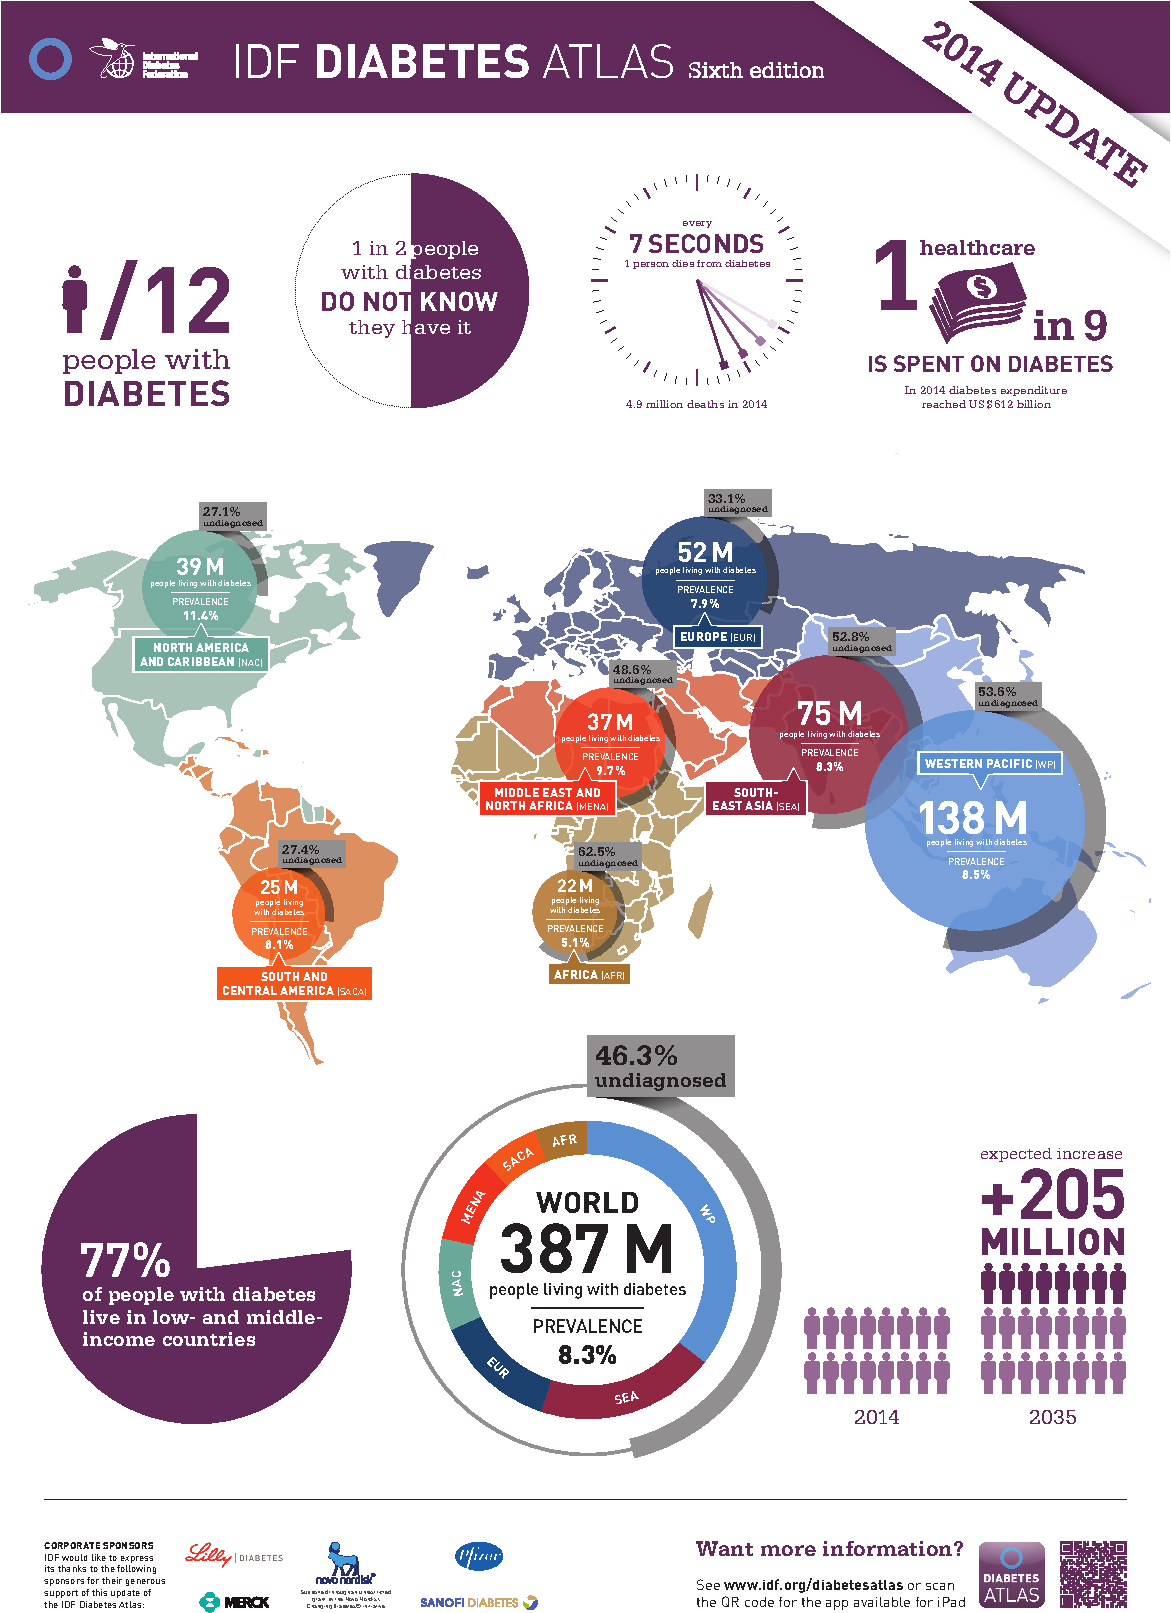
\includegraphics[width=\textwidth]{infogram-cropped.pdf}
  \caption{Diabetes atlas released by the International Diabetes Federation (IDF). Reuse of this material was granted by the IDF. The original is available at \url{http://www.idf.org/worlddiabetesday/toolkit/gp/facts-figures}.} 
  \label{intro:diabetes-infogram}
\end{figure}


%%%%%%%%%%%%%%%%%%%%%%%%%%%%%%%%%%%%%%%%%%%%%%%%
%      REGULATION OF BLOOD GLUCOSE LEVEL       %
%%%%%%%%%%%%%%%%%%%%%%%%%%%%%%%%%%%%%%%%%%%%%%%%

\subsection{Regulation of blood glucose levels}
To allow a better understanding of the underlying problems inherent to diabetes mellitus, we will briefly describe the critical role of insulin in the regulation of blood glucose levels.

Insulin is a peptide hormone which regulates the metabolism of fats, carbohydrates and proteins. In normal circumstances, insulin is released in response to changes in blood glucose concentration to prevent glucose levels from reaching toxic concentrations. Specifically, insulin promotes the absorption of glucose from the blood to skeletal muscles and fat tissue, thereby lowering the glucose level in the bloodstream, and additionally inhibits hepatic glucose output \citep{sonksen2000insulin}. Insulin is exclusively produced by pancreatic $\beta$ cells, which are located in clusters known as the islets of Langerhans. 

Hyperglycemia occurs when the regulation of the blood glucose level fails and hence toxic concentrations of glucose remain in the bloodstream. Such failures are typically caused by excessive glucose intake, insufficient insulin secretion and/or insulin resistance. 

%%%%%%%%%%%%%%%%%%%%%%%%%%%%%%%%%%%%%%%%%%%%%%%%
%         COMPLICATIONS AND COMORBIDITIES      %
%%%%%%%%%%%%%%%%%%%%%%%%%%%%%%%%%%%%%%%%%%%%%%%%

\subsection{Complications and comorbidities}
Exposure to chronic hyperglycemia can cause serious damage to many of the body's systems, including dysfunction and failure of various organs.

The leading complication of type 2 diabetes is cardiovascular disease, with about half of type 2 diabetes patient deaths attributable to a cardiovascular cause \citep{doi:10.1001/jama.2009.476, beulens2010global}. Microvascular complications also contribute considerably to the morbidity of the disease, specifically diabetes mellitus may lead to the progressive development of retinopathy (which potentially results in blindless), neuropathy (which can induce problems like foot ulcers), nephropathy (which can lead to renal failure) \citep{atkins2010diabetic} and small vessel vasculopathy causing lower extremity amputation \citep{beulens2010global}. Finally, patients with diabetes mellitus are at increased risk for peripheral vascular and cerebrovascular disease. 


% The global burden of diabetes and its complications: an emerging pandemic
% Cardiovascular disease (CVD) is the leading complication of type 2 diabetes and approximately one half of patients with type 2 diabetes will die of a cardiovascular cause. Angina, myocardial infarction, stroke, peripheral artery disease, and congestive heart failure are all common among patients with type 2 diabetes. IFG or IGT and the risks are further compounded by smoking, abnormal blood lipids, high blood pressure, and the other determinants of vascular risk established in nondiabetic populations [1,18].


% http://www.who.int/mediacentre/factsheets/fs312/en/
% What are common consequences of diabetes?
% Over time, diabetes can damage the heart, blood vessels, eyes, kidneys, and nerves.
% Diabetes increases the risk of heart disease and stroke. In a multinational study, 50% of people with diabetes die of cardiovascular disease (primarily heart disease and stroke) (6). Combined with reduced blood flow, neuropathy (nerve damage) in the feet increases the chance of foot ulcers, infection and eventual need for limb amputation. Diabetic retinopathy is an important cause of blindness, and occurs as a result of long-term accumulated damage to the small blood vessels in the retina. One percent of global blindness can be attributed to diabetes (7). Diabetes is among the leading causes of kidney failure (4). The overall risk of dying among people with diabetes is at least double the risk of their peers without diabetes (8).
% (2) World Health Organization. Global Health Estimates: Deaths by Cause, Age, Sex and Country, 2000-2012. Geneva, WHO, 2014. 
% (3) Mathers CD, Loncar D. Projections of global mortality and burden of disease from 2002 to 2030. PLoS Med, 2006, 3(11):e442.
% (4) Global status report on noncommunicable diseases 2010. Geneva, World Health Organization, 2011. 
% (5) Definition, diagnosis and classification of diabetes mellitus and its complications. Part 1: Diagnosis and classification of diabetes mellitus. Geneva, World Health Organization, 1999 (WHO/NCD/NCS/99.2). 
% (6) Morrish NJ, Wang SL, Stevens LK, Fuller JH, Keen H. Mortality and causes of death in the WHO Multinational Study of Vascular Disease in Diabetes. Diabetologia 2001, 44 Suppl 2:S14–S21.
% (7) Global data on visual impairments 2010. Geneva, World Health Organization, 2012.
% (8) Roglic G, Unwin N, Bennett PH, Mathers C, Tuomilehto J, Nag S et al. The burden of mortality attributable to diabetes: realistic estimates for the year 2000. Diabetes Care, 2005, 28(9):2130–2135.

%%%%%%%%%%%%%%%%%%%%%%%%%%%%%%%%%%%%%%%%%%%%%%%%%
%         CLASSIFICATION OF DIABETES            %
%%%%%%%%%%%%%%%%%%%%%%%%%%%%%%%%%%%%%%%%%%%%%%%%%

\subsection{Classification of diabetes mellitus}

Diabetes mellitus is a disorder of multiple etiologies and is subdivided into several more specific classes. The primary distinction between subclasses is essentially whether or not external insulin is necessary for survival. The first widely accepted classification was made by the World Health Organization (WHO) in 1980 \citep{WHO1980}, proposing two main classes of diabetes mellitus:
\begin{itemize}
\item \textbf{Type 1 diabetes (T1D)} refers to a condition characterized by insufficient insulin secretion caused by the autoimmune-mediated destruction of pancreatic $\beta$-cells. T1D patients require insulin for survival. T1D can start at an early age and has a strong genetic component.
\item \textbf{Type 2 diabetes (T2D)} results from defect(s) in insulin secretion, almost always paired with insulin resistance. T2D includes patients that require insulin for metabolic control and those that don't require insulin at all. The often asymptomatic onset of T2D typically occurs after 50 years of age\footnote{Though a case-study reported a 3 year-old child diagnosed with T2D at this year's European Association for the Study of Diabetes (EASD) meeting \citep[``\emph{A toddler with type 2 diabetes}'', pp. 152--153]{3yeardolddiabetic}.} and is often a result of genetic susceptibility combined with chronic obesity, a sedentary lifestyle and overly rich nutrition \citep{zimmet2001global, smyth2006diabetes}. Since obesity is such a common comorbidity of T2D \citep{smyth2006diabetes}, the terms \emph{diabesity} and \emph{obesity dependent diabetes mellitus} have been suggested \citep{shafrir1996development, astrup2000redefining}.
\end{itemize}
In the original proposal, T1D and T2D were aliased insulin-dependent diabetes mellitus (IDDM) and noninsulin-dependent diabetes mellitus (NIDDM), respectively \citep{WHO1980}. However, since then the WHO has deprecated the terms IDDM and NIDDM as their use frequently led to patients being classified based on treatment, rather than pathogenesis \citep{alberti1998definition}. Hence, contemporary terminology exclusively uses type 1 and type 2 to denote the main classes of diabetes mellitus. 

Though our work focuses on type 1 and particularly type 2 diabetes mellitus, it must be noted that more forms exist, such as gestational diabetes mellitus which may occur during pregnancy and then disappear or progress into T2D.

T2D accounts for over $90\%$ of diabetes patients and has long been considered an epidemic that affects both developing and developed nations \citep{zimmet1999diabetes,zimmet2001global,rocchini2002childhood,nathan2007impaired,chen2012worldwide, lam2012worldwide} effectively rendering it a pandemic \citep{beulens2010global}. T2D is often a manifestation of a much broader underlying disorder \citep{reaven1988role, zimmet1999diabetes}, including the \emph{metabolic syndrome} which is a cluster of cardiovascular disease risk factors that includes hyperinsulinemia, dislipidemia, hypertension, visceral obesity, hypercoagulability and microalbuminuria \citep{alberti2005metabolic, zimmet2001global, federation2010idf}. 

%%%%%%%%%%%%%%%%%%%%%%%%%%%%%%%%%%%%%%%%%%%%
%         PREVALENCE AND BURDEN            %
%%%%%%%%%%%%%%%%%%%%%%%%%%%%%%%%%%%%%%%%%%%%

\subsection{Prevalence and burden of diabetes}
The number of diabetes patients, particularly type 2 diabetes, is increasing rapidly. In developed countries, this increase is driven by population aging, lifestyle changes (particularly rising levels of obesity and inactivity) but also by greater longevity among diabetes patients \citep{stovring2003rising,beulens2010global}. The majority of social and economic burden of type 2 diabetes patients is attributable to vascular complications \citep{beulens2010global}, with pharmacy costs generating the majority of diabetes-related health expenditure \citep{nichols2002impact, gandra2006total}.

\paragraph{Prevalence} In 1995 an estimated 135 million people worldwide had diabetes, which has increased to 285 million patients worldwide in 2010 \citep{shaw2010global, chen2012worldwide} and is predicted by the WHO to increase further to at least 366 million by 2030 \citep{smyth2006diabetes}. WHO estimated the global prevalence of diabetes to be $9\%$ among adults over 18 years of age \citep{alwan2011global}. A recent study estimated the prevalence of diabetes in adults aged 20--79 in Belgium and Europe to be $8\%$ and $6.9\%$, respectively \citep{shaw2010global}. Typically, the prevalence of prediabetes is estimated even higher \citep{cowie2009full,yang2010prevalence,chen2012worldwide}.

\paragraph{Mortality} 
The premature mortality attributable to diabetes is widely underestimated because only a minority of persons with diabetes die from a cause that is uniquely attributable to the disease \citep{beulens2010global}. One study reported about 2.9 million deaths worldwide attributable to diabetes \citep{roglic2005burden} and indicated that this excess mortality accounts for over $8\%$ of deaths in developed countries. More recently, the global excess mortality in adults directly related to diabetes has been estimated to 3.8 million deaths \citep{beulens2010global}. The main causes of premature deaths in type 2 diabetes patients are due to cardiovascular and renal problems \citep{morrish2001mortality, beulens2010global}. 
Chapter~\ref{ch:survival} reports the survival of patients starting various glucose lowering pharmacotherapies in Belgium and confirms excess mortality in patients with diabetes compared to the general population. Additionally, our analysis indicates that the excess mortality is significantly associated with the type of pharmacotherapy, which is related to the patient's health status.


\paragraph{Cost} Managing diabetes and its complications is expensive, both to the affected individuals and healthcare systems around the world.  The International Diabetes Federation (IDF), estimates that diabetes already accounts for one ninth of the total healthcare budget in many countries in 2014 \citep{IDFfacts}. The IDF further reports an average cost per diabetes patient of 5,679 USD in Belgium \citep{IDFatlas}. Other sources report comparable numbers: the CoDiM study estimated that in Germany in 2001, annual direct mean costs per diabetic patient are $5,262$ EUR with an additional $5,019$ EUR indirect costs, compared to $2,755$ EUR and $3,691$ EUR for non-diabetics \citep{koster2006cost}. K\"oster et al. \citep{koster2006cost} also note that the direct costs of diabetic patients account for $14.2\%$ of total healthcare costs. Patients of type 2 diabetes with macrovascular complications generate costs that are three times higher than type 2 diabetes patients without macrovascular complications and seven times higher than people with neither type 2 diabetes nor macrovascular diseases \citep{beulens2010global}. The primary origin of diabetes-related healthcare expenditure are pharmacy costs \citep{nichols2002impact, gandra2006total}. The complications of diabetes constitute a large portion of the burden of the disease, with diabetes being a leading cause of blindness, lower limb amputation and kidney failure \citep{beulens2010global}. 


% http://europepmc.org/abstract/med/18350480
% http://download.springer.com/static/pdf/651/art%253A10.1007%252Fs00125-002-0860-3.pdf?originUrl=http%3A%2F%2Flink.springer.com%2Farticle%2F10.1007%2Fs00125-002-0860-3&token2=exp=1440768601~acl=%2Fstatic%2Fpdf%2F651%2Fart%25253A10.1007%25252Fs00125-002-0860-3.pdf%3ForiginUrl%3Dhttp%253A%252F%252Flink.springer.com%252Farticle%252F10.1007%252Fs00125-002-0860-3*~hmac=7111eff228db17edf0730fb32261e2f1d4a0400afbf88526eaa03e1bf6fe3f23
% http://informahealthcare.com/doi/abs/10.1185/030079905x65349
% http://cpr.sagepub.com/content/17/1_suppl/s3.full



\subsection{Treatment of diabetes mellitus} \label{intro:treatment}
%%%%%%%%%%%%%%%%%%%%%%%%%%%%%%%%%%%%
%%%%%%%%%%%%%%%%%%%%%%%%%%%%%%%%%%%%
%%%%%%%%%%%%%%%%%%%%%%%%%%%%%%%%%%%%
%%%%%%%v TODO   %%%%%%%%%%%%%%%%%%%%
%%%%%%%%%%%%%%%%%%%%%%%%%%%%%%%%%%%%
%%%%%%%%%%%%%%%%%%%%%%%%%%%%%%%%%%%%
%%%%%%%%%%%%%%%%%%%%%%%%%%%%%%%%%%%%
%%%%%%%%%%%%%%%%%%%%%%%%%%%%%%%%%%%%
%\todo{TODO prevention of complications http://www.nature.com/nature/journal/v414/n6865/full/414782a.html}
The fact chronic hyperglycemia may manifest in various ways is reflected in a wide variety of treatments for diabetes mellitus. Treatment of type 1 diabetes patients revolves around timely administration of external insulin, which they need for survival. In contrast, a wide range of treatment options exist for patients with type 2 diabetes.

Management of type 2 diabetes includes several lifestyle interventions, often specifically targetted towards weight loss, including healthy eating (specifically high-fiber, low-fat foods like fruits and vegetables), regular exercise and blood sugar monitoring and management. Pharmacotherapy via glucose lowering agents (GLAs) is used when lifestyle changes alone are insufficient for adequate glycemic control or when diabetes is already in a progressed stage at the time of clinical diagnosis. 

\newcommand{\regist}[1]{\emph{#1}\textsuperscript{\textregistered}}

We will elaborate on pharmacological treatment of type 2 diabetes, as this has played a crucial role in our work. Pharmacological therapies for (type 2) diabetes may be based on various biological mechanisms:
\begin{itemize}
\item \textbf{External insulin} is administered when insufficient insulin is secreted by the pancreas. External insulin is always necessary to treat type 1 diabetes but may also be required to treat insulin deficiency in type 2 diabetes. Insulin cannot be taken as a pill because it would be broken down during digestion just like protein in food. Instead, it must be injected or inhaled. \\
\item \textbf{Sensitizers} reduce the insulin resistance that is central in type 2 diabetes.
\begin{itemize}
        \item Biguanides suppress hepatic glucose output and increase uptake of glucose by the periphery. The most common agent in this class is \emph{metformin} (brand names include \regist{Glucophage}, \regist{Glucovance}) \citep{kirpichnikov2002metformin}. \\ % https://en.wikipedia.org/wiki/Metformin#Mechanism_of_action
        % https://en.wikipedia.org/wiki/Biguanide
        \item Thiazolidinediones (TZDs) enhance the effects of insulin by increasing insulin-dependent glucose disposal and reducing hepatic glucose output (as a result of increased hepatic insulin sensitivity) \citep{saltiel1996thiazolidinediones, yki2004thiazolidinediones}. 
        An example of TZDs is \emph{pioglitazone} (brand name \regist{Actos}). \\
\end{itemize}
\item \textbf{Secretagogues} increase insulin output from the pancreas. The main type of secretagogues -- sulfonylurea (SU) -- stimulate endogenous insulin secretion from pancreatic $\beta$-cells \citep{proks2002sulfonylurea}. Hypoglycemia is a major concern when using sulfonylureas \citep{bodmer2008metformin}.
        The most common SU are \emph{glimepiride} (brand name \regist{Amaryl}), \emph{glibenclamide} (\regist{Euglucon} and \regist{Daonil}), \emph{gliclazide} (\regist{Diamicron}), \emph{glipizide} (\regist{Glucotrol}) and \emph{gliquidone} (\regist{Glurenorm}). \\
        % https://en.wikipedia.org/wiki/Sulfonylurea
\item \textbf{Alpha-glucosidase inhibitors} slow down digestion of starch in the small intestine, thereby reducing the rate at which the resulting glucose enters the bloodstream. These agents do not have a direct effect on insulin secretion or sensitivity, but can (i) be sufficiently efficient in early stages of impaired glucose tolerance or (ii) be used in combination with other antidiabetic agents. 
A common alpha-glucosidase inhibitor is \emph{acarbose} (brand name \regist{Glucobay}). \\
\item \textbf{Incretin-based therapies} use the antidiabetic properties of the incretin hormone glucagon-like peptide 1 (GLP-1), namely that GLP-1 augments glucose-induced insulin secretion in a highly glucose-dependent manner \citep{nauck2009incretin,lovshin2009incretin}. As this form of insulin secretion occurs in a glucose-dependent manner, incretin-based therapies are less prone to cause hypoglycemia.
\begin{itemize}
        \item GLP-1 receptor agonists activate GLP-1 receptors, resulting in increased insulin synthesis and release \citep{drucker1987glucagon}. Common GLP-1 receptor agonists include \emph{liraglutide} (brand name \regist{Victoza}), \emph{exenatide} (\regist{Byetta}) and \emph{lixisenatide} (brand name \regist{Lyxumia}). \\
        \item Dipeptidyl peptidase-4 (DPP-4) inhibitors increase the blood concentration of GLP-1 by inhibiting its degradation caused by the enzyme DPP-4. Common DPP-4 inhibitors include \emph{sitagliptin} (brand name \regist{Januvia}), \emph{vildagliptin} (brand name \regist{Galvus}).  \\
\end{itemize}
\end{itemize} 

%Not all therapies are suitable for every patient, due to contraindications such as abnormal kidney function.+ statins, bitherapy, ...hypoglycemia


% http://www.hindawi.com/journals/ijvm/2012/918267/fig1/
% http://www.hindawi.com/journals/ijvm/2012/918267/

% http://www.nature.com/nm/journal/v12/n1/full/nm0106-75.html

\ifx
\subsection{Glucose level regulation as a state-space system}
With significant simplifications, we can summarize the glucose level regulatory mechanism as a dynamical system that is controlled via a basic feedback loop. This coarse approximation allows us to understand the main mechanisms of diabetes mellitus treatments on a mathematical level.

The system's states are $[glucose](t)$ and $[insulin](t)$ (concentrations) and its inputs are $\Delta glucose(t) \geq 0$ and $\Delta insulin(t) \geq 0$ which enter the bloodstream. 
\begin{itemize}
\item The glucose concentration is influenced negatively by the concentration of insulin ($A_{i\rightarrow g} < 0$) and positively by external input $\Delta glucose(t)$ ($B_g > 0$):
\begin{equation*}
\frac{d [glucose](t)}{d t} = A_{i\rightarrow g} [insulin](t) + B_g \Delta glucose(t)
\end{equation*}
\item The insulin concentration is influenced by insulin injection $\Delta insulin(t)$ and insulin secretion $\mathcal{S}_{insulin}(t)$, which in turn is influenced by the glucose level, i.e. $\mathcal{S}_{insulin}(t) = K[glucose](t)$ (with $K > 0$, $B_s > 0$ and $B_i > 0$):
\begin{align*}
\frac{d [insulin](t)}{d t} &= B_s \mathcal{S}_{insulin}(t) + B_i \Delta insulin(t), \\
        &= B_s K [glucose](t) + B_i \Delta insulin(t),
\end{align*}
where $B_i$ is a normalization based on volume and $K$ is a positive constant defining the amount of insulin secreted at a given glucose level.
\end{itemize}

This can be written as the following state-space system with two inputs:
\begin{align*}
\begin{bmatrix}
\frac{d [glucose]}{d t} \\
\frac{d [insulin]}{d t}
\end{bmatrix}
&= 
\begin{bmatrix}
0                    & A_{i\rightarrow g} \\
B_s K   & 0
\end{bmatrix}
\begin{bmatrix}
[glucose](t) \\
[insulin](t)
\end{bmatrix}
+
\begin{bmatrix}
B_g & 0 \\
0   & B_i
\end{bmatrix} 
\begin{bmatrix} 
\Delta glucose(t) \\
\Delta insulin(t)
\end{bmatrix}.
\end{align*}

Nature has somehow determined an optimal feedback gain $K^\star$ that usually works (or none of us would be here). The essential problems underlying diabetes can now be formalized as follows:
\begin{itemize}
\item Insufficient insulin secretion can be formalized as $K < K^\star$,
\item Insulin resistance can be formalized as $A_{i\rightarrow g} > A_{i\rightarrow g}^\star$.
\end{itemize}
Both of these effects imply a real control action that is smaller than optimal, directly leading to hyperglycemia. Treatment of diabetes mellitus generally attempts to do one of the following:
\begin{itemize}
\item   Decrease the amount of glucose entering the bloodstream.\\ 
        Equivalent to $\Delta glucose(t)\shortarrow{7}$.
\item   Increase insulin levels manually by injecting insulin, or increase secretion. \\ 
        Equivalent to $\Delta insulin(t)\shortarrow{1}$ and $K\shortarrow{1}$, respectively.
\item   Decrease insulin resistance in cells, to make them absorb glucose faster.\\ 
        Equivalent to $A_{i\rightarrow g}\shortarrow{7}$.
\end{itemize}

The approximated state-space system also indicates that for type 1 diabetes -- in which $\mathcal{S}_{insulin}(t)$ has a low saturation level -- treatments that attempt to increase insulin secretion or decrease insulin resistance are ineffective. Hence, treatment of type 1 diabetes requires insulin injections which explains its alias of insulin-dependent diabetes mellitus (IDDM).
\fi

\subsection{Secondary prevention of type 2 diabetes} \label{intro:screening}
%\paragraph{Secondary prevention of T2D is effective} 
Studies have convincingly shown that early detection and treatment of T2D can prevent or delay complications of the disease \citep{haffner1990cardiovascular,engelgau2000screening, genuth2003implications, holman200810, gaede2008effect, echouffo2011screening}. Additionally, treatment of early-stage T2D is often relatively simple and cheap (e.g. lifestyle changes, often specifically targetted towards weight loss) compared to the treatment of progressed T2D, which typically involves strict pharmacological therapy along with the treatment of potential complications \citep{pan1997effects,tuomilehto2001prevention,diabetes2002reduction,zammitt2005hypoglycemia}, indicating the value of secondary prevention.

%\paragraph{T2D is often diagnosed very late} 
Despite its widely-recognized importance, secondary prevention through screening for T2D proves to be problematic, as one fourth up to one third of T2D patients are estimated to be undiagnosed in developed countries \citep{diabetesliga, beagley2014global, american2014standards} and typically years pass between the onset of T2D and its clinical diagnosis \citep{harris1992onset}. In fact, the clinical diagnosis of T2D often follows signs of serious complications, which have developed during the latent stage of the disease \citep{rajala1998prevalence,harris2000early, hu2002elevated, american2014standards}. 

%\paragraph{Barriers for early detection of T2D} 
Diagnostic inertia for T2D arises in several ways. First, the disease may remain asymptomatic for many years \citep{alberti1998report}, during which unmanaged hyperglycemia may induce serious and irreversible development of micro -and macrovascular complications \citep{fowler2008microvascular, beagley2014global}. 
%Second, healthcare information related to a specific patient is often fragmented across databases of individual caregivers and other medical stakeholders, potentially causing situations in which various subtle symptoms of diabetes are presented to multiple caregivers, but the diagnosis remains elusive because each individual caregiver cannot see the big picture. 
Second, health and healthcare information related to a specific patient is often fragmented across databases of individual caregivers and other medical stakeholders. This can induce situations in which various subtle symptoms of diabetes are presented to multiple caregivers, but the diagnosis remains elusive because each individual caregiver receives too little information to spot the slumbering slayer.
Finally, universal screening for T2D is cost-prohibitive \citep{wareham2001should, engelgau2000screening}, though many organizations advise opportunistic screening of high-risk subgroups \citep{world1994prevention, alberti1998report, engelgau2000screening,american2014standards}.

Certain metabolic abnormalities typically precede T2D and can therefore be used as proverbial miners' canaries by screening approaches, specifically:
%Type 2 diabetes is typically preceded by the following metabolic abnormalities:
\begin{itemize}
\item \emph{Impaired fasting glucose (IFG)}, also known as prediabetes, is a condition in which fasting blood glucose levels are consistently higher than normal, but not high enough to warrant a diabetes diagnosis. Some patients with IFG can also be diagnosed with impaired glucose tolerance.
\item \emph{Impaired glucose tolerance (IGT)} is a prediabetic state of hyperglycemia which may precede T2D by many years. Patients with IGT exhibit raised glucose levels after 2 hours compared to healthy people, but not high enough to qualify for T2D. Patients with IGT present a higher risk for diabetes than patients with IFG. Approximately $40\%$ of subjects with IGT progress to diabetes over the next decade \citep{zimmet2001global}. Additionally, subjects with IGT have heightened risk of macrovascular disease compared to subjects with IFG \citep{tominaga1999impaired, unwin2002impaired}.
\end{itemize}
Both IFG and IGT are associated with insulin resistance and increased risk of diabetes and cardiovascular pathologies, with IGT being more strongly associated with cardiovascular outcomes \citep{unwin2002impaired}. Although the transition of IFG and/or IGT to diabetes may take many years, the majority of individuals with these pre-diabetic states eventually develop diabetes \cite{tuomilehto2001prevention,diabetes2002reduction,nathan2007impaired}. Additionally, the risk of complications is known to commence many years before the onset of clinical diabetes \cite{haffner1990cardiovascular,zimmet2001global}.

In the remainder of this Section we will discuss current diagnostic tests, existing screening programmes and the Belgian situation and recommendations.



\subsubsection{Diagnosis of diabetes} 
The gold standard to diagnose hyperglycemia is the oral glucose-tolerance test (OGTT), which determines how quickly glucose is cleared from the blood \citep{alberti1998definition, world2006definition}. In this test, patients are administered glucose after fasting for 12 hours and afterwards the patient's blood glucose levels are measured, sometimes at multiple intervals, but typically after 2 hours \citep{diabetesliga}.

Type 1 diabetes has a sufficiently pronounced clinical onset characterized by acute, extreme elevations in glucose concentrations combined with symptoms which make its diagnosis fairly undubious and typically timely \citep{international2009international}. Type 2 diabetes, however, has a more gradual onset making its diagnosis less straightforward and causing the diagnostic criteria to be debated regularly \citep{world2006definition, international2009international}.  The diagnostic criteria as currently recommended by the WHO are listed in Table~\ref{intro:who-diagnosis}.

The OGTT as diagnostic test was widely agreed upon, though in 2003 the American Diabetes Association (ADA) modified its recommendations in favor of using fasting plasma glucose to diagnose asymptomatic T2D \citep{world2006definition}. More recently, the use of the A1C assays for diagnosis was considered, though current point-of-care A1C assays were considered insufficiently accurate \citep{international2009international}.

\begin{table}[!h]
\colorbox{gray!20!white}{\parbox{\textwidth}{
\begin{itemize}
\item impaired fasting glucose (IFG):
\begin{itemize}
\item fasting plasma glucose $\geq 6.1$ and $< 7.0$ mmol/l, and
\item 2-hour plasma glucose $< 7.8$ mmol/l (if measured).
\end{itemize}
\item impaired glucose tolerance (IGT):
\begin{itemize}
\item fasting plasma glucose $< 7.0$ mmol/l, and
\item 2-hour plasma glucose $\geq 7.8$ and $< 11.1$ mmol/l.
\end{itemize}
\item diabetes:
\begin{itemize}
\item fasting plasma glucose $\geq 7.0$ mmol/l, or
\item 2-hour plasma glucose $\geq 11.1$ mmol/l.
\end{itemize}
\end{itemize}
}}
\caption{Diagnostic criteria for T2D as recommended by the WHO \citep{world2006definition}.} \label{intro:who-diagnosis}
\end{table}

\subsubsection{Existing screening approaches} \label{intro:screening-existing}
The clinical inertia in diagnosing type 2 diabetes is being tackled by a wide variety of screening approaches, which commonly rely on information that is already available or relatively easy to obtain. The main method to implement such screening methods is via questionnaires, possibly paired with clinical information such as parameters recorded in patients' electronic health records or by general practioners.

The Cambridge Risk Score (CRS) was developed to assess the probability of undiagnosed T2D based on data that is routinely available in primary care records, including age, sex, medication use, family history of diabetes, BMI and smoking status \citep{griffin2000diabetes}, The CRS and comparable scores have been shown to be useful on multiple occasions \citep{baan1999performance,griffin2000diabetes, park2002performance, spijkerman2004performance}. 
The FINDRISC score is based on a 10-year follow-up using age, BMI, waist circumference, history of antihypertensive drugs and high blood glucose, physical activity and diet and is used to predict drug-treated diabetes \citep{lindstrom2003diabetes}. The strongest reported predictors in this study were BMI, waist circumference, history of high blood glucose and physical activity. Gl{\"u}mer et al. \citep{glumer2004danish} developed a risk score based on age, sex, BMI, known hypertension, physical activity and family history of diabetes. The German diabetes risk score is based on age, waist circumference, height, history of hypertension, physical activity, smoking, and diet \citep{schulze2007accurate}.
More complex risk scores include various clinical parameters \citep{heikes2008diabetes, stern2002identification, mcneely2003comparison}.



%Simple questionnaires using only basic information can be a powerful tool to detect people that are at risk for diabetes, as proven in other countries [14–17].
%[14] Jaana Lindstr ̈om and Jaakko Tuomilehto. The diabetes risk score: a practical tool to predict type 2 diabetes risk. Diabetes Care, 26:725–731, 2003.
%[15] Charlotte Glumer, Bendix Carstensen, Annelli Sandbæk, Torsten Lauritzen, Torben Jørgensen, and Knut Borch-Johnsen. A danish diabetes risk score for targeted screening: the inter99 study. Diabetes Care, 27:727–733, 2004.
%[16] Caroline A. Baan, Johannes B. Ruige, Ronald P. Stolk, Jacqueline C.M. Witteman, Jacqueline M. Dekker, Robert J. Heine, and Edith J.M. Feskens. Performance of a predictive model to identify undiagnosed diabetes in a health care setting. Diabetes Care, 22:213–219, 1999.
%[17] Griffin SJ, Little PS, Hales CN, Kinmonth AL, and Wareham NJ. Diabetes risk score: towards earlier detection of type 2 diabetes in general practice. Diabetes Metab Res Rev, 16:164–171, 2000

%%%%%%%%%%%%%%%%%%%%%%%%%%%%%%%%%%%%%%%%%%%%%%%%%5
%
%		IN BELGIUM
%
%%%%%%%%%%%%%%%%%%%%%%%%%%%%%%%%%%%%%%%%%%%%%%%%%5


\subsubsection{Situation in Belgium} \label{intro:screening-belgium}
The IDF estimates over 170,000 undiagnosed diabetes patients in Belgium \citep{IDFatlas}. The Diabetes Liga estimates that currently one out of three T2D patients are undiagnosed, that one out of ten Belgians will have type 2 diabetes in 2030 and that $8\%$ and $6.5\%$ of the Belgian population currently has diabetes or prediabetes, respectively \citep{diabetesliga}. Domus Medica\footnote{A non-profit organization of general practionners that focuses on preventive medicine.} advises against population-wide screening, though it recommends case finding in high-risk subpopulations \citep{wens2005aanbeveling}, for instance via the risk factors listed in Table~\ref{intro:diabetes-liga-risk}.
\begin{table}[!h]
\colorbox{gray!20!white}{\parbox{\textwidth}{
\begin{itemize}
\item Persons of 18--45 years of age that meet one of the following conditions:
\begin{itemize}
\item prior history of gestational diabetes
\item prior history of stress-induced hyperglycemia
\end{itemize}
\item or two of the following conditions:
\begin{itemize}
\item prior history of giving birth to a baby of over 4.5 kg
\item diabetes in first-line relatives (mother, father, sister, brother)
\item BMI $\geq$ 25 kg/m$^2$
\item waist circumference $>88$ cm (for women) or $>102$ cm (for men)
\item treated for high blood pressure or with corticoids
\end{itemize}
\item Persons of 45--64 years of age that meet one of the conditions listed above.
\item Persons above 64 years old, regardless of additional risk factors.
\end{itemize}
}}
\caption{High-risk subpopulations according to the Diabetes Liga \citep{diabetesliga}.} \label{intro:diabetes-liga-risk}
\end{table}

The Belgian Scientific Institute of Public Health (WIV-ISP) reports that screening efforts are increasing in Belgium, but also indicates a need for risk stratification that goes beyond selecting all patients above a given age \citep{wivisp}.




% The onset of type 2 diabetes may occur up to 7 years before clinical diagnosis
% Harris MI, Klein R, Welborn TA, Knuiman MW. Onset of NIDDM occurs at least 4–7 years before clinical diagnosis. Diabetes Care 1992; 15:815–819. Cowie CC, Rus

% see also http://www.nature.com/nature/journal/v414/n6865/full/414782a.html

%The worldwide epidemiology of type 2 diabetes mellitus—present and future perspectives Lei Chen, Dianna J. Magliano and Paul Z. Zimmet
% The causes of the epidemic of T2DM are embedded in a very complex group of genetic and epigenetic systems interacting within an equally complex societal framework that determines behavior and environmental influences. This complexity is reflected in the diverse topics discussed in this Review. In the past few years considerable emphasis has been placed on the effect of the intrauterine environment in the epidemic of T2DM, particularly in the early onset of T2DM and obesity. Prevention of T2DM is a ‘whole-of-life’ task and requires an integrated approach operating from the origin of the disease.

% Full Accounting of Diabetes and Pre-Diabetes in the U.S. Population in 1988 –1994 and 2005–2006
% U.S. was 9.3%, of which 30% was undiagnosed based on fasting plasma glucos

% http://www.diabetesresearchclinicalpractice.com/article/S0168-8227(13)00384-7/abstract
% Globally, 45.8%, or 174.8 million of all diabetes cases in adults are estimated to be undiagnosed, ranging from 24.1% to 75.1% across data regions. An estimated 83.8% of all cases of UDM are in low- and middle-income countries. At a country level, Pacific Island nations have the highest prevalence of UDM.

% http://www.bettycjung.net/Pdfs/Alberti.pdf

% http://europepmc.org/abstract/med/18350480

% http://www.researchgate.net/profile/Leonor_Guariguata/publication/259153000_Global_estimates_of_undiagnosed_diabetes_in_adults_for_2013_for_the_IDF_Diabetes_Atlas/links/54f583fc0cf2ba61506653fb.pdf








%uit \citep{american2014standards}:
%Mass screening of asymptomatic individuals has not effectively identified those with prediabetes or diabetes, and rigorous clinical trials to provide such proof are unlikely to occur. In a large randomized controlled trial (RCT) in Europe, general practice patients between the ages of 40–69 years were screened for diabetes, then randomized by practice to routine diabetes care or intensive treatment of multiple risk factors. After 5.3 years of follow-up, CVD risk factors were modestly but significantly improved with intensive treatment. Incidence of first CVD event and mortality rates were not significantly different between groups \citep{griffin2011effect}. This study would seem to add support for early treatment of screen-detected diabetes, as risk factor control was excellent even in the routine treatment arm and both groups had lower event rates than predicted. The absence of a control unscreened arm limits the ability to definitely prove that screening impacts outcomes. Mathematical modeling studies suggest that screening, independent of risk factors, beginning at age 30 or 45 years is highly cost-effective \$11,000 per quality-adjusted life-year gained) \citep{kahn2010age}.




\section{Belgian mutual health insurance} \label{intro:health-insurance}
The Belgian health care insurance is a broad solidarity-based form of social insurance. Mutual health insurers are the legally-appointed bodies for managing and providing the Belgian compulsory health care and disability insurance. The Belgian sickness fund law of 1990 states that a main goal of mutualities is to promote the physical, psychological and social well-being of their members \citep{ziekenfondswet}.

Joining one of several mutual health insurers or, alternatively, the relief fund for sickness and disability insurance\footnote{In Dutch: Hulpkas voor Ziekte -en Invaliditeitsuitkering (HZIV).} is obliged for anyone who (i) starts working, (ii) is still studying at the age of 25 years or (iii) receives unemployment benefits. Among other things, mutual health insurers are responsible for refunding medical interventions, drug purchases and payments related to disability and pregnancy leave. To implement their operations, mutual health insurers dispose of large databases containing health expenditure records of all their respective members. 

This project was done in close collaboration with the National Alliance of Christian Mutualities (NACM).\footnote{In Dutch: Landsbond der Christelijke Mutualiteiten (LCM).} NACM  is the largest Belgian mutual health insurer with records of over 4.4 million persons and over 60\% and 40\% market share in Flanders and Belgium, respectively. All data extractions and analyses were done in-house at the department of medical management of NACM in its headquarters in Brussels under supervision of and upon request by the Chief Medical Officer.

We developed a screening system based exclusively on basic personal information (e.g. age, gender) and readily-available health expenditure records collected by NACM, without requiring any external input. The relevant patient-centric information embedded in these records belongs to three key classes:
\begin{itemize}
\item \textbf{Basic biographical information} includes the member's age, gender, place of residence and, if deceased, the date of death. Limited information regarding social status is also available, e.g. whether a member is entitled to increased compensation or suffers from a chronic illness.
\item \textbf{Medical provisions} are encoded via a national nomenclature comprising over 20,000 unique codes. Each medical act yields one or several of these nomenclature codes. 
\item \textbf{Drug purchases} are registered automatically and are encoded per package or per unit when purchased in retail and hospital pharmacies, respectively. In both cases, the encoding contains information about both volume and active substances. 
\end{itemize}

The time-stamped records related to provisions and drug purchases enable constructing a medical resource-use timeline for each patient. As this constitutes the main source of information in our work we will discuss claims records related to provisions and drug purchases in more detail in Sections~\ref{intro:interventions}~and~\ref{intro:drugs}. Finally, we will briefly discuss the overall quality of health expenditure data.


\subsection{Data related to medical interventions} \label{intro:interventions}
Each distinct medical intervention is encoded in a national nomenclature that is maintained by the National Institute for Health and Disability Insurance (NIHDI)\footnote{In Dutch: Rijksinstituut voor ziekte -en invaliditeitsverzekering (RIZIV).} \citep{van2008financing}. After a consultation, patients receive a certificate indicating which provisions were performed (a green, white or blue slip). The patient can then file a claim to get (partially) refunded through his or her mutual health insurer. Refunds can be claimed up to two years after the date of the intervention, though most patients do this more swiftly. In some cases, a copayment system enables the caregiver to get paid directly by the health insurer, removing the need for the patient to claim refunds.

The list of nomenclature numbers can be consulted via the website of the NIHDI and currently comprises over 20,000 unique codes. The sheer number of codes indicates the fine granularity at which medical interventions are encoded, making it a valuable source of information. Codes can fall out of use when interventions get deprecated or because they get replaced by other codes that are often more specific in some sense.

However, the codes that identify interventions only carry limited information. Specifically, these codes are sufficiently detailed to know which intervention was performed, but do not contain any information regarding its outcome. For example, there are codes indicating blood tests, but the results of these tests are not available to the mutual health insurer. As such, nomenclature codes often serve as proxies for specific diseases, but essentially carry no direct information regarding diagnoses, indications or clinical parameters.

\subsection{Data related to drug purchases} \label{intro:drugs}
Drug purchases work via a copayment system in Belgium, in which the patient only pays his or her share at the time of purchase while the rest is already deducted automatically. As such, drug purchases are automatically recorded and known to health insurers without requiring the patient to explicitly claim refunds and are therefore implicitly complete.

Each drug package carries a \emph{Code Nationale Kode} (CNK) code which indicates the volume in the package and information about the drug itself including its active substances. Hence, these CNK codes carry enough information to map a drug purchase onto one or several codes of the internationally used Anatomical Therapeutic Chemical (ATC) classification system with an associated amount of Defined Daily Doses (DDDs). Tables to map CNK codes onto ATC codes are provided freely by the BCFI\footnote{In Dutch: Belgisch Centrum voor Farmacotherapeutische Informatie.} and the APB\footnote{In Dutch: Algemene Pharmaceutische Bond.}.

The ATC classification system is maintained by the World Health Organization and divides active substances into different groups based on the organ or system on which they act and their therapeutic, pharmacological and chemical properties \citep{world1996guidelines}. Each drug is classified in groups at 5 levels in the ATC hierarchy: fourteen main groups (1st level), pharmacological/therapeutic subgroups (2nd level), chemical subgroups (3rd and 4th level) and the chemical substance (5th level). Figure~\ref{intro:atc-example} illustrates the structure of ATC system for common antidiabetic drugs.

\begin{figure}[!h]
\dirtree{%
.1 \textsc{A}: alimentary tract and metabolism.
.2 \textsc{A10}: drugs used in diabetes.
.3 \textsc{A10A}: {\color{blue}insulins} and analogues.
.3 \textsc{A10B}: blood glucose-lowering drugs, excluding insulins.
.4 \textsc{A10BA}: {\color{blue}biguanides}.
.5 \textsc{A10BA02}: {\color{red}metformin}.
.4 \textsc{A10BB}: {\color{blue}sulfonylureas}.
.5 \textsc{A10BB01}: {\color{red}glibenclamide}.
.5 \textsc{A10BB08}: {\color{red}gliquidone}.
.5 \textsc{A10BB12}: {\color{red}glimepiride}.
.4 \textsc{A10BF}: {\color{blue}alpha-glucosidase inhibitors}.
.5 \textsc{A10BF01}: {\color{red}acarbose}.
.4 \textsc{A10BG}: {\color{blue}thiazolinediones}.
.5 \textsc{A10BG03}: {\color{red}pioglitazone}.
.4 \textsc{A10BH}: {\color{blue}dipeptidyl peptidase 4 (DPP-4) inhibitors}.
.5 \textsc{A10BH01}: {\color{red}sitagliptin}.
.5 \textsc{A10BH02}: {\color{red}vildagliptin}.
}
\caption{Example of the ATC hierarchy for common GLAs. A brief explanation of these different active substances is given in Section~\ref{intro:treatment}.} \label{intro:atc-example}
\end{figure}


\subsection{Quality of health expenditure data}
Overall, health expenditure data can be considered complete, due to the clear financial incentive for patients and caregivers to file claims. The automated registration of drug purchases also contributes to this aspect.

A key benefit of Belgian health expenditure data is that it integrates resource-use from all medical sources. Patients may consult multiple caregivers and institutions but each patient can only be affiliated to one mutual health insurer at a given moment in time. Additionally, most Belgians never switch mutual health insurer.

Health expenditure records give a fine-grained overview of patients' medical histories thanks to the detailed encoding of provisions and drug packages. However, the absence of data related to outcomes, diagnoses and clinical parameters constitutes an important limitation. In this regard, it must be noted that a lot of relevant information to screen for T2D is missing, such as glycated hemoglobin levels, lifestyle, BMI and potential genetic predisposition.

Health expenditure records prove extremely useful for retrospective observational studies, as is common in epidemiology. However, a certain lag exists between medical acts  and the appearance of associated records in health expenditure databases. For provision records, the maximum lag is two years, while for drug purchases the lag is less than half a year. These lags present problems for applications that require quasi real-time information, such as disease outbreak detection, but are less problematic for screening.

A disadvantage is that expenditure data may be noisy. Most sources of noise can be considered random and hence neglected, but some structural issues exist as well. A specific example is fraud through \emph{upcoding}, which refers to caregivers that wilfully report wrong nomenclature codes, or codes corresponding to provisions that were never performed, in order to obtain higher refunds. This phenomenon is known to plague healthcare systems in various countries and likely occurs in Belgium as well to some extent \citep{silverman2004medicare,steinbusch2007risk,berta2010effects}.

Finally, it is worth noting that the potential of health expenditure data for clinical applications is also being investigated in other countries. A highly visible recent example was the Heritage Health Prize competition to identify patients who will be admitted to a hospital within the next year using historical claims data, with an impressive \$3,000,000 prize pool.\footnote{More information is available at \url{http://www.heritagehealthprize.com/}.}



%%%%%%%%%%%%%%%%%%%%%%%%%%%%%%%%%%%%%%%%%%%%%%%%%%%
%               MACHINE LEARNING
%%%%%%%%%%%%%%%%%%%%%%%%%%%%%%%%%%%%%%%%%%%%%%%%%%%

\section{Machine learning challenges and contributions} \label{intro:machine-learning}
This Section highlights the main machine learning contributions made during this project. We will briefly describe the fundamental problems that were tackled, outline the approach and clarify how it fits into the overarching theme of identifying patients at risk for diabetes based on health expenditure data. Chapters~\ref{ch:ensemblesvm}~to~\ref{ch:diabetesjmlr} describe the solutions and methodologies we developed in detail.

We approached the screening task as a binary classification problem. Binary classifiers are models which yield some level of confidence that an instance belongs to the positive class, based on the features of that instance. In our application, every patient represents an instance. Each patient is either diabetic (positive) or non-diabetic (negative). The biographic information and resource-use history of each patient represent the associated features.

The relationships between all aspects of this project's machine learning research are depicted in Figure~\ref{fig:ml-structure}. Our contributions revolved around three focal points: learning from positive and unlabeled data, automated hyperparameter optimization and the development of reusable open-source software to facilitate reproducibility. Sections~\ref{intro:pulearning}~to~\ref{intro:software} describe each focal point in more detail.

\begin{figure}[!h]
\centering
\resizebox{\textwidth}{!}{
\begin{tikzpicture}[mindmap,
  every node/.style={font=\large},
  every concept/.style={minimum size=3cm, text width=3cm, fill=none, very thick},
  level 1 concept/.append style={level distance=150,sibling angle=120}]

  \begin{scope}[mindmap, text=black, minimum size=3cm]
    \node [concept, minimum size=4cm, color=black, text=black] at (0, 0) (diabetesjmlr) {\Large{\textbf{Diabetes Screening Chapter \ref{ch:diabetesjmlr}}}}
	[clockwise from=90, level distance=130] 
	child[concept color=green!50!black] {node [concept, text=black, fill=green!50!black, fill opacity=0.2, text opacity=1] at (-0.5, -0.2) (pulearning) {\Large{\textbf{Semi-supervised Learning}}}
		[clockwise from=0, sibling angle=180]
		child {node [concept] at (1.7, -0.4) (resvm) {Robust PU learning with SVM models \\ Chapter \ref{ch:resvm}}}
		child {node [concept] at (-5.6, 0.7) (evaluation) {Evaluating models without known negatives \\ Chapter \ref{ch:evaluation}}}
	      }
	child[concept color=cyan!80!black] {node [concept, text=black, fill=cyan!80!black, fill opacity=0.2, text opacity=1] at (0.8, -0.2) (software) {\Large{\textbf{Open-Source \\ Software}}}
		[clockwise from=200, level distance=200, sibling angle=90]
		child {node [concept] at (-1.2, -1.5) (optunity) {Optunity \\ Chapter \ref{ch:optunity}}}
		child {node [concept] at (3.2, 2.4) (esvm) {EnsembleSVM \\ Chapter \ref{ch:ensemblesvm}}}
	      }
	child[concept color=red!80!black]{node [concept, text=black, fill=red!80!black, fill opacity=0.2, text opacity=1] at (-1.1, 1.3) (tuning) {\Large{\textbf{Hyper-parameter Search}}}
		[clockwise from=270, level distance=200, sibling angle=90]
		child {node [concept] at (2.4, -1.1) (mic) {Optimization challenges \\ Chapter \ref{ch:mic2015}}}
	      };
  \end{scope}

%\path (resvm) to[circle connection bar switch color=from (cyan!80!black) to (red!80!black)] (esvm) ;
\path (tuning) to[circle connection bar switch color=from (red!80!black) to (cyan!80!black)] (optunity) ;
%\path (mic) to[circle connection bar switch color=from (red!80!black) to (cyan!80!black)] (optunity) ;
\path (tuning) to[circle connection bar switch color=from (red!80!black) to (green!50!black)] (evaluation) ;

\tikzset{>={Latex[width=3mm,length=3mm]}}

\draw[dotted, ->, ultra thick, color=gray, shorten >= 1mm, shorten <= 1mm] (evaluation) to[bend right=11] (optunity) ;
\draw[dotted, ->, ultra thick, color=gray, shorten >= 1mm, shorten <= 1mm] (optunity) to[bend right=5] (resvm) ;
\draw[dotted, ->, ultra thick, color=gray, shorten >= 1mm, shorten <= 1mm] (esvm) to[bend left=30] (resvm) ;
\draw[dotted, ->, ultra thick, color=gray, shorten >= 1mm, shorten <= 1mm] (mic) to[bend left=10] (optunity) ;
\draw[dotted, ->, ultra thick, color=gray, shorten >= 1mm, shorten <= 1mm] (optunity) to[bend left=10] (mic) ;

\draw[dotted, ->, ultra thick, color=gray, shorten >= 1mm, shorten <= 1mm] (resvm) -> (diabetesjmlr) ;
\draw[dotted, ->, ultra thick, color=gray, shorten >= 1mm, shorten <= 1mm] (evaluation) -> (diabetesjmlr) ;
\draw[dotted, ->, ultra thick, color=gray, shorten >= 1mm, shorten <= 1mm] (optunity) -> (diabetesjmlr) ;
\draw[dotted, ->, ultra thick, color=gray, shorten >= 1mm, shorten <= 1mm] (esvm) -> (diabetesjmlr) ;

\end{tikzpicture}
}
\caption{Dependencies of the key contributions made to machine learning research during this project. To enable diabetes screening based on Belgian health expenditure data (Chapter~\ref{ch:diabetesjmlr}), we made contributions to semi-supervised learning (Chapters \ref{ch:resvm} and \ref{ch:evaluation}), automated hyperparameter search (Chapters \ref{ch:mic2015} and \ref{ch:optunity}) and open-source machine learning software (Chapters \ref{ch:ensemblesvm} and \ref{ch:optunity}).} \label{fig:ml-structure}
\end{figure}

\subsection{Learning from positive and unlabeled data} \label{intro:pulearning}
A critical challenge inherent to our application is an infeasibility to ascertain which patients are non-diabetic based only on health expenditure records. This problem originates from several sources, most notably because a significant fraction of diabetic patients is undiagnosed (as discussed in Section~\ref{intro:screening}) and additionally because initial diabetes therapies may exclusively consist of lifestyle changes (cfr. Section~\ref{intro:treatment}) which are not recorded in health expenditure data. 

Fortunately, we were able to identify a reasonable set of known diabetics (positives) based on health expenditure data. Positives were identified via the use of GLA therapy over extended periods of time. The thus identified set of positives mainly consists of patients with progressed diabetes (since the treatment involves pharmacotherapy) and omits patients with (potentially diagnosed) prediabetes. It must be noted that this labeling induces some false positives, mainly due to the use of GLA medication for alternative reasons (e.g. use of metformin for weight loss).

Given these labeling issues, we had to learn binary classifiers from positive and unlabeled data to enable screening based exclusively on health expenditure data. This learning scenario is receiving increasing amounts of research attention and is commonly dubbed PU learning. During this project, we improved an existing PU learning method and additionally developed a method to evaluate classifiers without known negatives. The latter aspect is particularly important because it has significant practical implications and was previously uncharted territory.

\subsubsection{Building classifiers with only positive and unlabeled data} 
This is a common topic within semi-supervised learning, presenting additional complexity compared to fully supervised binary classification.\footnote{In this context, fully supervised means all class labels are known.} Various methods have been devised to cope with the increased uncertainty, based on one of two fundamental approaches:
(i) first attempt to infer a set of likely negatives from the unlabeled data and then train a fully supervised model to distinguish known positives from inferred negatives \citep{liu02partially,Yu:2005:SCM:1108759.1108762,Li03learningto} vis-\`a-vis (ii) treat unlabeled instances as negatives with noisy class labels and deal with this directly \citep{Elkan:2008:LCO:1401890.1401920,Lee03learningwith,Liu:2003:BTC:951949.952139,MORDELET-2010-523336,Liu:2005:PSC:2138033.2138052}.

The method we developed fits into the latter category and is described in detail in Chapter~\ref{ch:resvm}. Our technique achieves state-of-the-art performance in PU learning and is additionally designed for robustness against false positives, which are known to exist in our application. False positives significantly deteriorate the performance of other existing methods, limiting their usability in our project.

\subsubsection{Evaluating classifiers with only positive and unlabeled data} 
Assessing the performance of binary classifiers without known negatives was an open problem at the start of the project. Prior to our work, a few methods have been devised for model selection in PU learning which allow basic pairwise comparisons between classifiers \citep{lee2003learning}. During our work, some additional related methods were developed by others \citep{sechidis2014statistical, hajizadeh2014evaluating}. However, none of these quantify the performance of a given classifier in terms of commonly used metrics like sensitivity, specificity and area under the ROC curve.

The performance of models for screening must be quantified before their use can even be considered, however no convincing method to quantify performance without known negatives existed. To circumvent this problem we initially considered manually obtaining negative labels by directly asking patients whether or not they had diabetes. Clearly, this is a very sensitive matter and would additionally have been labour intensive to acquire a sufficient amount of negative labels. 

Instead of manual labeling, we developed a method to reliably estimate performance of binary classifiers without known negatives (cfr. Chapter~\ref{ch:evaluation}). This method is the first of its kind and relies only on the reasonable assumption that known positives are sampled completely at random from all positives, which implies that the distributions of known and latent positives are comparable. Our work effectively reduces estimating performance without negatives to estimating the fraction of positives in the unlabeled set, which is often feasible.

\subsection{Automated hyperparameter optimization} \label{intro:tuning}
Most machine learning algorithms are parameterized, for example to allow the user to determine an optimal model complexity for a given problem. The coefficients of a trained model are commonly called parameters, and hence the parameters used to describe the training problem itself are referred to as \emph{hyper}parameters. Current research focuses on automatically determining suitable values for these hyperparameters \citep{hutter2009paramils, bergstra2011algorithms, snoek2012practical, bergstra2012random, bergstra2013hyperopt, eggensperger2013towards, thornton2013auto}, which essentially boils down to the development of suitable (heuristic) optimizers.

Some of the key challenges in hyperparameter optimization are described in Chapter~\ref{ch:mic2015}. Several libraries have been developed to automate this process and have proven to be far more efficient than manual tuning or grid search \citep{hutter2009paramils, bergstra2012random, snoek2012practical, bergstra2013hyperopt}. However, most of these libraries are challenging to install (even for seasoned programmers!) and feature a lot of complex configurations, hence effectively limiting their potential userbase to experts. To fill this apparant gap of user-friendly tuning software, we have developed a cross-platform open-source Python library that provides a variety of suitable optimizers to automate hyperparameter search via a simple, lightweight API. This library is described in Chapter~\ref{ch:optunity}.


\subsection{Open-source software} \label{intro:software}
Machine learning research requires high-quality, tested and documented software to advance rapidly. Fortunately, several authoraties in the machine learning field are appreciative of open-source software \citep{sonnenburg2007need}. Overall, the field is blessed with a wealth of open-source packages covering all aspects of the learning process and we strongly feel that cultivating this ecosystem is in the best interest of the entire academic community, for reasons such as efficiency, reliability and reproducibility. It is worth noting that every analysis in this project was done using freely available software.

As we recognize the value and importance of a solid open-source ecosystem, we decided to pay it forward by developing two open-source libraries of our own: \emph{EnsembleSVM} and \emph{Optunity}.

\paragraph{EnsembleSVM} is a C++ package for ensemble learning with support vector machine (SVM) base models. This software enables efficiently computing nonlinear models on large-scale data sets, which would otherwise be infeasible without significant computational resources. The PU learning method we developed (cfr. Chapter~\ref{ch:resvm}) is a use-case of EnsembleSVM and was implemented entirely using the API offered by the library. EnsembleSVM is described in Chapter~\ref{ch:ensemblesvm}.

\paragraph{Optunity} is a Python library for automated hyperparameter optimization, with interfaces to R, MATLAB, Octave and Java. An overview of Optunity is given in Chapter~\ref{ch:optunity}. At the time of writing, Optunity receives roughly 1,000 downloads monthly via the Python Package Index (PyPI). Optunity was used to optimize the hyperparameters of the learning approaches we used to construct models for diabetes screening.


%%%%%%%%%%%%%%%%%%%%%%%%%%%%%%%%%%%%%%%%%%%%%%%%%%%
%               OUTLINE
%%%%%%%%%%%%%%%%%%%%%%%%%%%%%%%%%%%%%%%%%%%%%%%%%%%

\section{Structure of the thesis} \label{intro:structure}
This Section summarizes the content of all subsequent chapters  and reiterates how every aspect is relevant to diabetes screening based on Belgian health expenditure records.

\newcommand{\chapteritem}[2]{\item \emph{Chapter~\ref{ch:#1}} #2}
\begin{itemize}

\chapteritem{survival} describes a study we performed to quantify the survival of Belgian patients after starting various glucose-lowering pharmacotherapies. Unlike other studies, our study does not focus on relative efficacy of different GLA therapies. Instead, it is the only one that provides an expected survival rate for patients starting a specific therapy, accounting for all possible future therapies commonly seen in the Belgian population.

\chapteritem{ensemblesvm}{introduces the EnsembleSVM software package, which provides efficient routines for ensemble learning using SVM base models.}

\chapteritem{resvm}{describes a novel algorithm to learn robust binary classifiers from positive and unlabeled data. The key design criterion is robustness to false positives, which was lacking in existing approaches. The implementation is based on EnsembleSVM (see Chapter~\ref{ch:ensemblesvm}).}

\chapteritem{mic2015}{discusses the main optimization challenges posed by automated hyperparameter search and summarizes the current state-of-the-art.}

\chapteritem{optunity}{describes the Optunity software package, which provides metaheuristic optimization routines for automated hyperparameter optimization. Optunity is available on most commonly used machine learning platforms and tackles the challenges outlined in Chapter~\ref{ch:mic2015}.}

\chapteritem{evaluation}{presents a method to evaluate the performance of binary classifiers without negative labels. This method enables estimating most commonly used performance metrics in a semi-supervised setting, which was uncharted territory.}

\chapteritem{diabetesjmlr}{integrates all machine learning aspects into a workflow to predict which patients are likely to start glucose-lowering pharmacotherapy, based exclusively on readily available, individual health expenditure records. This chapter combines all techniques described in previous chapters.}

\end{itemize}



%%%%%%%%%%%%%%%%%%%%%%%%%%%%%%%%%%%%%%%%%%%%%%%%%%
% Keep the following \cleardoublepage at the end of this file, 
% otherwise \includeonly includes empty pages.
\cleardoublepage

% vim: tw=70 nocindent expandtab foldmethod=marker foldmarker={{{}{,}{}}}

\section{Background and definitions}
We first review the relevant background on model evaluation and issues caused by partial labeling. 

%%%%%%%%%%%%%%%%%%%%%%%%%%%%%%%%%%%%%%%%%%%%%%%%
%%%
%		RANK DISTRIBUTIONS

%%%
%%%%%%%%%%%%%%%%%%%%%%%%%%%%%%%%%%%%%%%%%%%%%%%%

\subsection{Rank distributions and contingency tables} \label{contingency-intro}
%Many classifiers assign each example a numeric \emph{decision value} during prediction. This is a measure of confidence that the instance belongs to the positive class, e.g. logistic regression yields the associated probability ($\hat{y}\in [0, 1]$) and SVM classifiers yield a signed distance to the separating hyperplane ($\hat{y} \in \mathbb{R}$). Any binary classifier can be described as a functional $\mathcal{C}$ that maps input vectors $\mathbf{x}\sim\inputspace$ onto the real line, i.e. $\mathcal{C}:\inputspace \mapsto \mathbb{R}$. Higher decision values imply higher confidence that the instance belongs to the positive class. 

We focus on binary decision problems, where the goal is to classify examples as either positive or negative. Most learned models (e.g., SVM, logistic regression, naive Bayes) predict a numeric score for each example where higher values imply higher confidence that the instance belongs to the positive class. Typically, a \emph{ranking} $\overall$ is produced by sorting examples in descending order by their numeric score such that confident positive predictions are ranked close to the top of $\overall$.\footnote{Which means a low value for rank in this work, though this is often referred to as \emph{highly ranked} in literature.}  

%$\rank(\overall, x)$ denotes the rank of an instance $x$ in $\overall$.


%\emph{decision value} to each example during prediction. Intuitively, the decision value represents the confidence that the instance belongs to the positive class. Typically, higher decision values imply higher confidence that the instance belongs to the positive class. 


 %The rank of an instance is defined by its position in $\overall$, such that confident positive predictions (characterized by high decision values) are ranked close to the top of $\overall$.\footnote{Which means a low value for rank in this work, though this is often referred to as \emph{highly ranked} in literature.}

Within a ranking $\overall$, we treat $\pos \subset \overall$ as the subset of examples with positive labels, $\bar{\pos} = \overall - \pos$  as the subset of examples with negative labels, and let $\rank(\overall, x)$ denote the rank of an instance $x$ in $\overall$.  Given a cutoff rank $r,$ predictions can be made by assigning the positive class to the $r$ top ranked instances and the negative class to the rest. This decision rule yields a \emph{true positive rate (TPR)}, which is the fraction of positive examples that are correctly labeled as positive, and \emph{false positive rate (FPR)}, which is the fraction of negative examples that are incorrectly labeled as positive:
\begin{align}
\TPR(\pos, r) &= \probability(\rank(\overall, x) \leq r\ |\ x \in \pos), \nonumber \\
	      &= |\{\ x \in \pos\ :\ \rank(\overall, x) \leq r\}|\ /\ |\pos|, \label{tpr-def} \\
\FPR(\pos, r) &= \probability(\rank(\overall, \bar{x}) \leq r\ |\ \bar{x} \in \bar{\pos}) = \TPR(\overall - \pos, r). \label{fpr-def}
\end{align}
\noindent Given the number of positives $|\pos|$ and negatives $|\overall-\pos|$, the contingency table for a rank $r$ is: \\
\begin{minipage}[c]{0.45\textwidth}
\begin{align}
\TP(\pos,r) &= \TPR(\pos, r) \cdot |\pos|, \label{tp-def} \\
\FN(\pos,r) &= |\pos| - \TP(\pos, r), 
\end{align}
\end{minipage}\hfill\begin{minipage}[c]{0.52\textwidth}
\begin{align}
\FP(\pos,r) &= \FPR(\pos, r) \cdot |\overall-\pos|, \nonumber \\
\TN(\pos,r) &= |\overall-\pos| - \FP(\pos,r). %= (1 - \FPR(\pos, r)) \cdot |\overall - \pos| \\
\end{align}
\end{minipage}

The rank distribution of a set of instances $\pos$ within an overall ranking $\overall$ is defined as the distribution of their corresponding ranks within $\overall$. The rank cumulative distribution function (CDF) of a set of instances $\pos$ is defined as the (empirical) CDF of their ranks, i.e. $\forall\ r \in \{1,\ldots,|\overall|\}$:
\begin{equation}
\cdf{\pos}{r} = \probability(\rank(\overall, x) \leq r \ |\ x \in \pos). \label{rankcdf}
\end{equation}
The concept of rank CDF is illustrated in Figure~\ref{fig:rank-cdf}. Note that $ \cdf{\pos}{r} \equiv \TPR(\pos, r) $ (Equations~\eqref{tpr-def} and~\eqref{rankcdf}), that is, the rank CDF of the set of positives $\pos$ at rank $r$ in an overall ranking $\overall$ can be interpreted directly as a true positive rate, when labeling the $r$ top ranked instances as positive.
%%%%%%%%% HACK TO MAKE EVERYTHING FIT %%%%%%%%
%%%%%%%%%%%%%%%%% END OF HACK %%%%%%%%%%%%%%%%
\begin{figure}[ht]
  \centering
  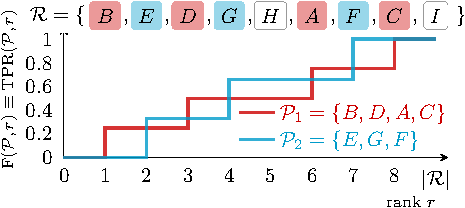
\includegraphics[width=0.6\textwidth]{rank-cdf.pdf}
  \caption{Rank CDF of two sets of positives $\pos_1 = \{B, D, A, C\}$ and $\pos_2=\{E, G, F\}$ within an overall ranking $\overall=\{B,E,D,G,H,A,F,C,I\}$, with $|\pos_1|=4$ and $|\pos_2|=3$. In practice $\overall$ is obtained by sorting the data according to classifier score. The rank CDF of a set $\mathcal{S}\subseteq \mathcal{R}$ is based on the positions of elements of $\mathcal{S}$ in $\overall$. } 
  \label{fig:rank-cdf}
\end{figure}

We use two convenience functions to partition sets of ranks:
\begin{align*}
\topfun(X, \ranksymb) &= \{\ \rank(\overall, x) \leq \ranksymb\ :\ x \in X\ \}, \\
\bottomfun(X, \ranksymb) &= \{\ \rank(\overall, x) > \ranksymb\ :\ x \in X\ \},
\end{align*}
such that $\topfun(X,\ranksymb)\ \cup\ \bottomfun(X,\ranksymb) = X$ and $|\topfun(X,r)| = \cdf{X}{\ranksymb}\cdot |X|$. 

%%%%%%%%%%%%%%%%%%%%%%%%%%%%%%%%%%%%%%%%%%%%%%%%
%%%
%		ROC CURVES
%%%
%%%%%%%%%%%%%%%%%%%%%%%%%%%%%%%%%%%%%%%%%%%%%%%%

\subsection{ROC and PR curves} \label{roc}
Receiver operator characteristic (ROC) curves are used extensively for evaluating classifiers in machine learning \citep{Bradley:1997:UAU:1746432.1746434} as they illustrate the performance of a model over its entire operating range. ROC curves depict how a model's true positive rate (shown on the y-axis) varies as a function of its false positive rate (shown on the x-axis). Each cutoff rank $r \in \{1,\ldots,|\overall|\}$ corresponds to a single point (i.e., (FPR, TPR) pair) in ROC space (Eqs.~\eqref{tpr-def} and \eqref{fpr-def}). An (empirical) ROC curve for a ranking $\overall$ and set of positives $\pos \subset \overall$ is constructed by computing $\FPR(\pos, r)$ and $\TPR(\pos, r)$ at each rank $r$ and interpolating by drawing a straight line between points corresponding to consecutive ranks.  
The area under an ROC curve (AUROC) is a commonly used summary statistic, typically ranging between $0.5$ (random model) and $1$ (perfect model). AUROC is a popular  criterion in model selection and is often used as the optimization objective in hyperparameter search \citep{Bradley:1997:UAU:1746432.1746434}.

%ROC curves are insensitive to changes in the distribtuion of because FPR and TPR are each based on a single column of a contingency table \citep{fawcett2006introduction}. ROC curves can also be used for cost-sensitive learning \citep{provost1997analysis}. %and can be used for cost-sensitive learning.

%The area under an ROC curve (AUROC) is a commonly used summary statistic which typically ranges between $0.5$ (random model) and $1$ (perfect model). AUROC is equal to the probability that a random positive is ranked higher than a random negative, which is equivalent to the Wilcoxon test of ranks \citep{hanley1982meaning}. It is a popular criterion to optimize during hyperparameter search \citep{lessmann2008benchmarking, DBLP:journals/corr/ClaesenSPMM14}.


Precision-Recall (PR) curves  \citep{davis2006relationship} are an alternative to ROC curves that show how a model's precision (y-axis) varies as a function of recall (x-axis). Recall is equivalent to TPR and precision is the fraction of examples classified as
positive that are truly positive ($\TP / (\TP+\FP)$). PR curves are widely used when there is a skew in the class distributions~\cite{davis-icml09,claesen2014robust}.



%Algorithm 2 has a clear advantage over Algorithm 1. This difference exists because in this domain the number of negative examples greatly exceeds the number of positives examples. Consequently, a large change in the number of false positives can lead to a small change in the false positive rate used in ROC analysis

%were originally used in information retrieval \citep{raghavan1989critical}. PR curves visualize the evolution of precision ($\TP / (\TP+\FN)$) versus recall (TPR) and can be used as an alternative to ROC curves to assess classifier performance.

%%%%%%%%%%%%%%%%%%%%%%%%%%%%%%%%%%%%%%%%%%%%%%%%
%%%
%		PARTIAL LABELING
%%%
%%%%%%%%%%%%%%%%%%%%%%%%%%%%%%%%%%%%%%%%%%%%%%%%

\subsection{Evaluation with partially labeled data}
In the partial labeling setting, $\overall$ consists of disjoint sets of known positives $\knownpos$, known negatives $\knownneg$ and unlabeled instances $\unlabeled$. %, i.e., $\overall = \knownpos \cup \knownneg \cup\ \unlabeled$.
The unlabeled set $\unlabeled$ consists of latent positives $\latentpos$ and latent negatives. The fraction of latent positives in the unlabeled set plays a crucial role in our work, denoted by $\beta$:
\begin{equation}
\pfrac = \probability(x \in \latentpos\ |\ x \in \unlabeled) = |\latentpos|\ /\ |\unlabeled|. \label{pfrac} %\frac{|\latentpos|}{|\unlabeled|}. \label{pfrac}
\end{equation}
%We assume an estimate $\hat{\pfrac} \approx \pfrac$ is available. This can be obtained via direct statistical estimates based on training data \citep{Elkan:2008:LCO:1401890.1401920} or domain knowledge, e.g. in disease screening $\hat{\pfrac}$ is the prevalence of undiagnosed patients of the disease \citep{holmberg1996estimated, rathmann2003high}.

Note that computing contingency tables requires fully labeled data. If only a few labeled instances of both classes are available, they can be used to compute rough estimates of predictive performance. However, if only positive labels are available, even a rough approximation of common metrics cannot be estimated directly as we do not know which unlabeled examples are positives and which are negative. A common approach to evaluate models in a PU learning context is to treat the full unlabeled set as negative \citep{mordelet2011prodige,sifrim2013extasy,sechidis2014statistical}, though we will show that this may lead to spurious results. 

%This approach is inherently pessimistic: at any cutoff rank, the FPR is overestimated and the TPR is underestimated because all latent positives are treated as negative. Hence, this method is only useful when $\pfrac$ is small, that is, $\pfrac < 0.01$ as its bias is related to $\pfrac/\hat{\pfrac}$. This is particularly problematic for PR curves, as we will show later. \todo{rewrite last 3 phrases}

%Trivial best and worst case bounds on performance are easily obtained by considering all latent positives to be ranked at the top or bottom of the unlabeled set, respectively. However, these are too wide for any meaningful use when $|\latentpos| \gg |\knownpos|$, which is a common situation in practice.

%We focus on the PU learning setting, in which only positive labels are available, i.e. $\knownneg = \emptyset$, though our approach can include known negatives too (incorporating known negatives is explained in Theorem~\ref{main-theorem} and Section~\ref{contingency}).

%Computing contingency tables and performance curves based on an overall ranking $\overall$ as described in Sections~\ref{contingency-intro} and \ref{roc} requires a known set of \emph{all} positives $\pos_\Omega = \knownpos \cup \latentpos$. Since $\latentpos$ is unknown, they cannot be computed directly. Section~\ref{rank-roc} details how to tackle this problem theoretically and Section~\ref{practical} describes a practical approach.



%\subsection{Performance curves from partially labeled data}
%If only a few labeled instances of both classes are available, they can be used to construct a rough estimate of either the ROC or PR curve. However, if only positive labels are available, even a rough approximation of the ROC or PR curve cannot be estimated directly. 

%In PU learning, a simple approach is to treat the full unlabeled set as negative, i.e., assume $\hat{\pfrac} = 0$. This approach is inherently pessimistic: at any cutoff rank, the FPR is overestimated and the TPR is underestimated because all latent positives are treated as negative. Hence, this method is only useful when $\pfrac$ is small, that is, $\pfrac < 0.01$ as its bias is related to $\pfrac/\hat{\pfrac}$. This is particularly problematic for PR curves, as we will show later.

%Trivial best and worst case bounds on performance are easily obtained by considering all latent positives to be ranked at the top or bottom of the unlabeled set, respectively. However, these are too wide for any meaningful use when $|\latentpos| \gg |\knownpos|$, which is a common situation in practice.

%\floatsetup[figure]{capposition=bottom}
\section{Relationship between the rank CDF of positives and contingency tables} \label{rank-roc}
The challenge of incorporating unlabeled data into an evaluation metric is knowing which unlabeled examples are latent positives and which are latent negatives. Our insight is that, if the known positives are sampled completely at random from all positives, the rank distribution of latent positives should follow the rank distribution of known positives. Thus if we know $\pfrac$, which is needed to compute the expected number of latent positives within the unlabeled data, this provides an avenue for building contingency tables that incorporate the unlabeled data. To do so, we first prove relationships between rank CDFs of sets of positives within an overall ranking at a given rank $r$ and the corresponding contingency tables. Then, we use these relationships to prove bounds on the FPR at a given rank $r$ when the ranking includes unlabeled examples, some of which are latent positives. 

%The challenge of incorporating unlabeled data into an evaluation metric is knowing which unlabeled examples are latent positives and which are latent negatives. Our insight is that, if the known positives are a random sample from all positives, the rank CDF of the latent positives should follow the rank distribution of the known positives. This assumes that we know $\beta$ as we need to compute the expected number of latent positives within the unlabeled data. To do so, we first prove relationships between the rank CDFs of sets of positives within an overall ranking at a given rank $r$ and the corresponding contingency table. Then, we use these relationships to prove bounds on the FPR at a given rank $r$ when the ranking includes unlabeled examples, some of which are latent positives. 

%These relationships allow us to efficiently estimate contingency tables based on an overall ranking $\overall$, a subset of known positives $\knownpos$ and an estimate $\hat{\pfrac}$ in Section~\ref{practical}. 

%%%%%%%%%%%%%%%%%%%%%%%%%%%%%%%%%%%%%%%%%%%%%%%%%%
% 	LEMMA RANK -> FPR
%%%%%%%%%%%%%%%%%%%%%%%%%%%%%%%%%%%%%%%%%%%%%%%%%%

\subsection{Rank distributions and contingency tables based on subsets of positives within a ranking}
We begin by considering given sets of positives within an overall ranking. Proofs of all lemmas can be found in Appendix~\ref*{proofs}, along with figures to illustrate the associated property.

\begin{replemma}{lemma-rank-fpr}
Given a rank $\ranksymb$ and two disjoint subsets of positives $\pos_1$ and $\pos_2$ within an overall ranking $\overall$. If $|\pos_1|=|\pos_2|$ and $\TPR(\pos_1, \ranksymb) > \TPR(\pos_2,\ranksymb)$, then $\FPR(\pos_1,\ranksymb) < \FPR(\pos_2,\ranksymb)$.
\end{replemma}


%%%%%%%%%%%%%%%%%%%%%%%%%%%%%%%%%%%%%%%%%%%%%%%%%%
% 	LEMMA RANK UNION
%%%%%%%%%%%%%%%%%%%%%%%%%%%%%%%%%%%%%%%%%%%%%%%%%%

\begin{replemma}{lemma-rank-union}
Given a rank $\ranksymb$ and two disjoint sets of positives $\pos_1$, $\pos_2$ in a ranking $\overall$ and $\bothpos=\pos_1\cup\pos_2$. If $\TPR(\pos_1,\ranksymb) < \TPR(\pos_2, \ranksymb)$ then $\TPR(\pos_1,\ranksymb) < \TPR(\bothpos,\ranksymb) < \TPR(\pos_2, \ranksymb)$.
\end{replemma}

\begin{repcorollary}{corollary-rank-union}
Given a rank $\ranksymb$ and three sets of positives $\pos_A$, $\pos_B$ and $\pos_C$ within a ranking $\overall$ such that $\pos_A\cap\pos_B=\emptyset$ and $\pos_A\cap\pos_C=\emptyset$ and $|\pos_B|=|\pos_C|$, then
\begin{equation*}
\TPR(\pos_B,\ranksymb) < \TPR(\pos_C,\ranksymb) \quad\leftrightarrow\quad \TPR(\pos_A\cup \pos_B,\ranksymb) < \TPR(\pos_A\cup\pos_C,\ranksymb).
\end{equation*}
%\textbf{Proof}: all terms are equal for $\TPR(\pos_A\cup \pos_B,\ranksymb)$ and $\TPR(\pos_A\cup \pos_C,\ranksymb)$ except $\tprsymb_B < \tprsymb_C$ in Eq.~\eqref{tpr-union}.
\end{repcorollary}

% TODO
\ifx
\begin{figure}[!h]
  \centering
  \RawFloats
  \begin{minipage}[b]{0.49\textwidth}
  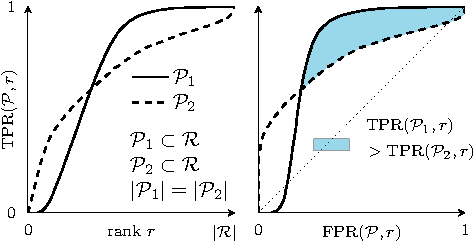
\includegraphics[width=\textwidth]{lemma_rank_fpr.pdf}
  \caption{Illustration of Lemma~\ref{lemma-rank-fpr}: higher TPR at a given rank $r$ implies lower FPR at $r$ for two positive sets of the same size.}
  \label{fig:lemma-rank-fpr}
  \vfill
  \end{minipage}
  \hfill
%\end{figure}
%\end{minipage}
%\begin{minipage}[0.47\textwidth}
%\begin{figure}[!h]
%  \centering
  \begin{minipage}[b]{0.49\textwidth}
  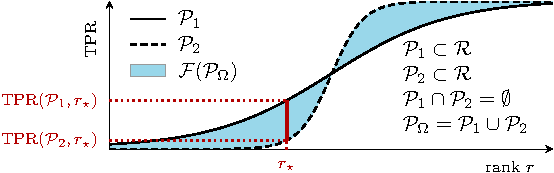
\includegraphics[width=\textwidth]{lemma-rank-union.pdf}
  \caption{Illustration of Lemma~\ref{lemma-rank-union}: $\mathcal{F}(\cdot)$ denotes feasible region. The rank distribution of the union $\bothpos$ of two sets of positives $\pos_1$ and $\pos_2$ lies between their respective rank distributions.} 
  \label{fig:lemma-rank-union}
\vfill
  \end{minipage}
\end{figure}
%\end{minipage}
\fi

\subsection{Contingency tables based on partially labeled data}
Lemmas~\ref*{lemma-rank-fpr} and \ref*{lemma-rank-union} describe relationships between rank distributions and contingency tables of different (but known) sets of positives within an overall ranking. 
%However, computing contingency tables from partially labeled data requires accounting for the unknown set of latent positive examples $\latentpos$ in the unlabeled data, that is, $\bothpos = \knownpos \cup \latentpos$, such that $|\latentpos| > 0$ and $|\latentpos|=\pfrac\cdot|\unlabeled|$. 
We now show how to construct contingency tables corresponding to the greatest-lower and least-upper bound of the FPR at a given rank, accounting for the unknown set of latent positive example from partially labeled data, given $\pfrac$. 

%Assuming a known proportion of latent positive examples in the unlabeled data, 

%and prove that one corresponds to the greatest lower bound of the FPR and the other corresponds to the least upper bound of the FPR at a specified rank.  

%Assumming a known proportion of latent positive examples in the unlabeled data, we now show to construct two contingency tables from partially labeled data and prove that one corresponds to the greatest lower bound of the FPR and the other corresponds to the least upper bound of the FPR at a specified rank.  

%%%%%%%%%%%%%%%%%%%%%%%%%%%%%%%%%%%%%%%%%%%%%%%%%%
% 	THEOREM
%%%%%%%%%%%%%%%%%%%%%%%%%%%%%%%%%%%%%%%%%%%%%%%%%%

\begin{theorem} \label{main-theorem}
%Given an overall ranking $\overall = \knownpos \cup \knownneg \cup \unlabeled$, consisting of disjoint sets of known positives $\knownpos$, known negatives $\knownneg$ and unlabeled instances $\unlabeled$, where $\unlabeled$ contains an unknown set of latent positives $\latentpos \subset \unlabeled$ of known size $|\latentpos| = \pfrac \cdot|\unlabeled|$. Given a rank $\ranksymb$ and an upper bound $\mathcal{T}_{ub}(\ranksymb) \geq \TPR(\latentpos, \ranksymb)$, a tight lower bound on $\FPR(\bothpos, \ranksymb)$ with $\bothpos = \knownpos \cup \latentpos$ can be found without explicitly identifying $\latentpos$.
Given an overall ranking $\overall$ consisting of disjoint sets of known positives $\knownpos$, known negatives $\knownneg$ and unlabeled instances $\unlabeled$, where $\unlabeled$ contains an unknown set of latent positives $\latentpos \subset \unlabeled$ of known size $|\latentpos| = \pfrac \cdot|\unlabeled|$. Given a rank $\ranksymb$ and an upper bound $\mathcal{T}_{ub}(\ranksymb) \geq \TPR(\latentpos, \ranksymb)$, a tight lower bound on $\FPR(\bothpos, \ranksymb)$ with $\bothpos = \knownpos \cup \latentpos$ can be found without explicitly identifying $\latentpos$.


\textbf{Proof}: Step 1: assign a set of surrogate positives $\surrpos$:\footnote{A surrogate positive is an example that we treat as if its ground truth label is positive (even though in reality its ground truth label is unknown) when constructing a contingency table.}
\begin{align}
\surrpos = &\argmin_{\surrposopt\subset\ \unlabeled}\ \TPR(\surrposopt, \ranksymb), \label{eq:surrpos-def}  \\ 
&\subjectto\ \TPR(\surrposopt,\ranksymb) \geq \mathcal{T}_{ub}(\ranksymb) \text{ and } |\surrposopt|=\pfrac\cdot|\unlabeled|, \nonumber
\end{align}
then $\TPR(\surrpos,\ranksymb) \geq \TPR(\latentpos,\ranksymb)$ by construction. If $|\topfun(\unlabeled, r)| < \pfrac\mathcal{T}_{ub}(\ranksymb)\cdot |\unlabeled|$, then no $\surrpos$ exists that satisfies the constraint $\TPR(\surrpos, \ranksymb) \geq \mathcal{T}_{ub}(\ranksymb)$ in Equation~\eqref{eq:surrpos-def}.\footnote{An infeasibility implies that $\mathcal{T}_{ub}(\ranksymb)$ and/or $\pfrac$ are too high.} In this case, treat all instances in $\topfun(\unlabeled, \ranksymb)$ as surrogate positive, which trivially implies $\TPR(\surrpos, \ranksymb) \geq \TPR(\latentpos, \ranksymb)$.

Step 2: define $\bothposapprox = \knownpos \cup \surrpos$. Using Corollary~\ref{corollary-rank-union} yields $\TPR(\bothposapprox, \ranksymb) \geq \TPR(\bothpos, \ranksymb)$. Since $|\bothposapprox|=|\bothpos|$, using Lemma~\ref*{lemma-rank-fpr} yields the lower bound on FPR, i.e., $\FPR(\bothposapprox, \ranksymb) \leq \FPR(\bothpos, \ranksymb)$.\hfill$\blacksquare$
%\begin{align*}
%\FPR(\bothposapprox, \ranksymb) \leq \FPR(\bothpos, \ranksymb).\tag*{$\blacksquare$}
%\end{align*}
\end{theorem}

Applying Theorem~\ref{main-theorem} yields a nontrivial lower bound on $\FPR(\bothpos,\ranksymb)$. In Lemma~\ref*{lemma-glb} we prove that $\FPR(\bothposapprox,\ranksymb)$ is the greatest achievable lower bound based on a given $\unlabeled\subset\overall$.

\begin{replemma}{lemma-glb}
Minimizing $\TPR(\surrpos, \ranksymb)$ in Equation~\eqref{eq:surrpos-def} of Theorem~\ref{main-theorem} ensures $\FPR(\bothposapprox, \ranksymb)$ is the greatest achievable lower bound on $\FPR(\bothpos, \ranksymb)$ given $\pfrac$, $\mathcal{T}_{ub}(\ranksymb)$, $\overall$ and $\unlabeled$. 
\end{replemma}

Due to its symmetry, Theorem~\ref{main-theorem} can also be used to obtain the least achievable upper bound of $\FPR(\bothpos, \ranksymb)$ given a ranking $\overall$ and a bound $\mathcal{T}_{lb}(\ranksymb) \leq \TPR(\surrpos, \ranksymb)$ by assigning $\surrpos$ such that:
\begin{align}
\surrpos = &\argmax_{\surrposopt\subset\ \unlabeled}\ \TPR(\surrposopt, \ranksymb), \label{eq:surrpos-def-ub} \\
&\subjectto\ \TPR(\surrposopt,\ranksymb) \leq \mathcal{T}_{lb}(\ranksymb) \text{ and } |\surrposopt|=\pfrac\cdot|\unlabeled| \nonumber. 
\end{align}
%If this is infeasible (implying $\mathcal{T}_{ub}(\ranksymb)$ and/or $\pfrac$ are too low), use 
%\begin{equation*}
%\surrpos = \argmin_{\surrpos\subset\ \unlabeled} \TPR(\surrpos, \ranksymb). \label{eq:surrpos-alternative}
%\end{equation*}

\section{Efficiently computing the bounds} \label{practical}


%Theorem~\ref{main-theorem} and Lemma~\ref{lemma-glb} provide a constructive approach to compute contingency tables based on partially labeled data, corresponding to a greatest lower bound and least upper bound on $\FPR(\bothpos,\ranksymb)$. In Section~\ref{rank-roc} we assumed to have bounds on $\TPR(\latentpos,\ranksymb)$ and a known fraction of latent positives in $\unlabeled$.

%We now describe the practical details for using Theorem~\ref{main-theorem} and Lemma~\ref{lemma-glb} to compute the contingency tables corresponding to the greatest lower bound and least upper bound on $\FPR(\bothpos,\ranksymb)$ from a finite sample. First, we propose an efficient method to compute contingency tables via Theorem~\ref{main-theorem}. Second, we describe how to obtain bounds on $\mathcal{T}_{lb}(\ranksymb)$ and $\mathcal{T}_{ub}(\ranksymb)$ that are needed for building the contingency table.  

We now describe how to use Theorem~\ref{main-theorem} and Lemma~\ref*{lemma-glb} to compute the contingency tables corresponding to the greatest lower and least upper bound on $\FPR(\bothpos,\ranksymb)$ from a finite sample. First, we explain how to compute contingency tables efficiently via Theorem~\ref{main-theorem}. Second, we propose how to obtain the bounds on rank CDF ($\mathcal{T}_{lb}(\ranksymb)$ and $\mathcal{T}_{ub}(\ranksymb)$) that are needed to build the contingency table.  


%%%%%%%%%%%%%%%%%%%%%%%%%%%%%%%%%%%%%%%%%%%%%%%%
%%%
%		CONTINGENCY TABLES
%%%
%%%%%%%%%%%%%%%%%%%%%%%%%%%%%%%%%%%%%%%%%%%%%%%%

\subsection{Computing the contingency table with greatest-lower bound on FPR at given rank $r$} \label{contingency}
Given $\pfrac$, $\overall$ and the sets $\knownpos$, $\knownneg$, and $\unlabeled$, Theorem~\ref{main-theorem} enables computing contingency tables corresponding to the least upper and greatest lower bound on FPR at a given cutoff rank $r$. We focus on building the contingency table corresponding to the lower bound on the FPR, the other is analogous. %Estimating the contingency table for an upper bound on the FPR is analogous. 

%First, 



%The proof of Theorem~\ref{main-theorem} involves identifying a set of surrogate positives $\surrpos$ in the unlabeled data. 
%Because the full rank distribution of $\surrpos$ is not necessary to compute the contingency table at rank $\ranksymb$, it is not needed to explicitly construct the set of surrogate positives. The only requirement is that the ranks in $\surrpos$ are distributed such that $\TPR(\surrpos,\ranksymb) \geq \mathcal{T}_{ub}(\ranksymb)$ where $\mathcal{T}_{ub}(\ranksymb)$ is an upper bound on $\TPR(\latentpos,\ranksymb)$ (Section~\ref{quantile-bounds} describes a method to compute $\mathcal{T}_{ub}(\ranksymb)$).
%

%To construct a contingency table at a given cutoff rank $r$, we decompose the computation to consider the labeled and unlabeled instances separately: 
%\begin{equation*}
%\left[\begin{matrix}
%\TP_{\Omega}^r & \FP_{\Omega}^r\\
%\FN_{\Omega}^r & \TN_{\Omega}^r
%\end{matrix}\right] = 
%\left[\begin{matrix}
%\TP_{L}^r & \FP_{L}^r\\
%\FN_{L}^r & \TN_{L}^r
%\end{matrix}\right]
%+
%\left[\begin{matrix}
%\TP_{U}^r & \FP_{U}^r\\
%\FN_{U}^r & \TN_{U}^r
%\end{matrix}\right].
%\end{equation*}

We decompose the computation to consider the labeled and unlabeled instances separately: 
\begin{equation*}
\resizebox{\textwidth}{!}{$
\begin{bmatrix}
\TP_{\Omega}^r & \FP_{\Omega}^r \\
\FN_{\Omega}^r & \TN_{\Omega}^r
\end{bmatrix} = 
\begin{bmatrix*}[l]
\TP_{L}^r = |\topfun(\knownpos, r)| & \FP_{L}^r = |\topfun(\knownneg, r)|\\
\FN_{L}^r = |\bottomfun(\knownpos, r)| & \TN_{L}^r = |\bottomfun(\knownneg, r)|
\end{bmatrix*}
+
\begin{bmatrix}
\TP_{U}^r & \FP_{U}^r\\
\FN_{U}^r & \TN_{U}^r
\end{bmatrix}$.}
\end{equation*}
Given that at rank $r$ we can directly compute partial contingency tables for the labeled data based on $\overall$, $\knownpos$ and $\knownneg$, we focus on computing the contingency table for the unlabeled instances. 

%where 
Given $\mathcal{T}_{ub}(r)$, we can use Theorem~\ref{main-theorem} to determine the values in the contingency table for the unlabeled instances for the greatest lower bound on FPR. Doing so requires inferring a set of surrogate positives $\surrpos$ from the unlabeled data, which must be a solution to Equation~\eqref{eq:surrpos-def}. This requires $\theta$ surrogate positives in $\topfun(\surrpos,\ranksymb)$ and the rest in $\bottomfun(\surrpos,\ranksymb)$, where $\theta$ is defined as:
\begin{equation}
\theta = \ceil{\mathcal{T}_{ub}(r) \cdot |\surrpos|} = \ceil{\mathcal{T}_{ub}(r) \cdot \pfrac \cdot |\unlabeled|}, \label{theta}
\end{equation}
By rounding up in Equation~\eqref{theta}, we ensure that $\TPR(\surrpos, r) \geq \mathcal{T}_{ub}(r)$ as required by Theorem~\ref{main-theorem}. 

In practice, two corner cases must be considered. One is if $|\topfun(\unlabeled,\ranksymb)| < \theta$, then it is impossible to assign $\theta$ surrogates below rank $\ranksymb$ in $\unlabeled$. In this case, all of $\topfun(\unlabeled,\ranksymb)$ is assigned as surrogate positives and the remaining surrogates are in $\bottomfun(\unlabeled,\ranksymb)$ (as discussed in Theorem~\ref{main-theorem}). 
Two is if $|\bottomfun(\unlabeled, r)| < |\surrpos| - \theta$, in which case all of $\bottomfun(\unlabeled, r)$ is labeled positive and the remaining surrogate positives inevitably end up in $\topfun(\unlabeled, r)$. Hence, any set of surrogate positives $\surrpos$ that meets the following criteria solves Equation~\eqref{eq:surrpos-def} and thus yields a valid bound:
\begin{align}
|\surrpos| &= \pfrac \cdot |\unlabeled|, \nonumber \\
|\topfun(\surrpos,r)| &= 
\left\{\begin{matrix*}[l] 
\min\big(|\topfun(\unlabeled, r)|,\ \theta\big) &\text{if } |\surrpos|-\theta \leq |\bottomfun(\unlabeled, r)|, \\
|\surrpos| - |\bottomfun(\unlabeled, r)| &\text{if } |\surrpos|-\theta > |\bottomfun(\unlabeled, r)|.
\end{matrix*}\right. \label{eq:surrpos-conditions}
\end{align}

Given a set of surrogate positives $\surrpos$, the partial contingency table of interest becomes:
\begin{equation}
\begin{bmatrix}
\TP_{U}^r & \FP_{U}^r\\
\FN_{U}^r & \TN_{U}^r
\end{bmatrix} = 
\begin{bmatrix*}[l]
|\topfun(\surrpos,\ranksymb)| 		& |\topfun(\unlabeled-\surrpos,\ranksymb)|\\
|\bottomfun(\surrpos,\ranksymb)| 	& |\bottomfun(\unlabeled-\surrpos,\ranksymb)|
\end{bmatrix*}, \label{eq:partial-ct-unlabeled}
\end{equation}
where $\unlabeled-\surrpos$ is the set of surrogate negatives and $|\surrpos|$ and $|\topfun(\surrpos,r)|$ are known via Eq.~\ref{eq:surrpos-conditions}. 

%Note that we only need set sizes to compute this partial contingency table. Furthermore, the required sizes of $|\surrpos|$ and $|\topfun(\surrpos, r)|$ are known based on the conditions in Equation~\eqref{eq:surrpos-conditions}. Hence, computing this partial contingency table can be done very efficiently without even explicitly identifiying the set of surrogate positives $\surrpos$.

Note that computing the partial contingency table for the unlabeled data can be done very efficiently since it only requires set sizes as shown in Equation~\ref{eq:partial-ct-unlabeled}, without explicitly partitioning the unlabeled set $\unlabeled$. That is, we do not need to know which examples are in $\topfun(\surrpos,r)$, $\bottomfun(\surrpos,r)$, $\topfun(\unlabeled-\surrpos,r)$ and $\bottomfun(\unlabeled-\surrpos,r)$, we just need to know the number of examples each set contains.


%Note that computing the partial contingency table for the unlabeled data can be done very efficiently as it only requires set sizes: the number of true positives (i.e., $|\topfun(\surrpos,\ranksymb)|$), the number false negatives (i.e., $|\bottomfun(\surrpos,\ranksymb)|$), and the total number of unlabeled examples. That is, we do not need to know which examples are in $\topfun(\surrpos,r)$, just the number of examples it contains.

%To obtain the greatest lower bound on FPR via Theorem~\ref{main-theorem} we must compute a contingency table based on surrogate positives $\surrpos$, where $\surrpos$ is obtained via Equation~\eqref{eq:surrpos-def}. This translates into requiring $\theta$ surrogate positives in $\topfun(\surrpos,\ranksymb)$ and the rest in $\bottomfun(\surrpos,\ranksymb)$, where:
%\begin{equation}
%\theta = \ceil{\mathcal{T}_{ub}(r) \cdot |\surrpos|} = \ceil{\pfrac\mathcal{T}_{ub}(r) \cdot |\unlabeled|}, \label{theta}
%\end{equation}
%By rounding up in Equation~\eqref{theta}, we ensure that $\TPR(\surrpos, r) \geq \mathcal{T}_{ub}(r)$ as required by Theorem~\ref{main-theorem}. 

%However, it is not necessary to explicitly construct sets of surrogate positives because the full rank distribution of $\surrpos$ is not needed to compute the contingency table at rank $\ranksymb$. The only requirement is that the ranks in $\surrpos$ are distributed such that $\TPR(\surrpos,\ranksymb) \geq \mathcal{T}_{ub}(\ranksymb)$ where $\mathcal{T}_{ub}(\ranksymb)$ is an upper bound on $\TPR(\latentpos,\ranksymb)$ (Section~\ref{quantile-bounds} describes computing $\mathcal{T}_{ub}(\ranksymb)$).





 


%\paragraph{Partial contingency table based on labeled instances} \ \newline
%We can directly compute partial contingency tables based on $\overall$, $\knownpos$ and $\knownneg$ at given rank $r$:

%\begin{minipage}[c]{0.9\textwidth}
%\centering
%\begin{minipage}[c]{0.6\textwidth}
%\begin{align*}
%\knownpos \rightarrow \TP_{L}^r &= |\topfun(\knownpos, r)|, \\
%	\FN_{L}^r &= |\bottomfun(\knownpos, r)|, 
%\end{align*}
%\end{minipage}
%\begin{minipage}[c]{0.3\textwidth}
%\begin{align*}
%\knownneg \rightarrow \FP_{L}^r &= |\topfun(\knownneg, r)|, \\
%	\TN_{L}^r &= |\bottomfun(\knownneg, r)|.
%\end{align*}
%\end{minipage}
%\end{minipage}

%\paragraph{Partial contingency table based on unlabeled instances} \ \newline
%The partial contingency table from $\unlabeled$ can be determined based on $\TPR(\knownpos, r)$, $\unlabeled$ and $\pfrac$. To obtain an upper bound in ROC space (i.e. a lower bound on FPR for a given TPR) via Theorem~\ref{main-theorem}, we must compute a contingency table corresponding to surrogate positive labels $\surrpos \subset \unlabeled$, such that $|\surrpos| = \pfrac\cdot |\unlabeled|$ and $\mathcal{R}_\tprsymb(\surrpos) \leq \mathcal{R}_\tprsymb(\knownpos)$ where $\tprsymb = \TPR(\knownpos, r)$. This can be done as follows:
%\begin{equation}
%\theta = \ceil{\TPR(\knownpos, r) \cdot |\surrpos|}, \label{theta}
%\end{equation}
%where $\theta$ represents the desired number of surrogate positives ranked higher than $r$ (i.e. within $\topfun(\surrpos, r)$). By rounding up in Equation~\eqref{theta}, we ensure that $\TPR(\surrpos, r) \geq \TPR(\knownpos, r)$ which implies $\mathcal{R}_\tprsymb(\surrpos) \leq \mathcal{R}_\tprsymb(\knownpos)$ at $\tprsymb=\TPR(\knownpos, r)$.

%The proof of Theorem~\ref{main-theorem} requires creating sets of surrogate positives $\surrpos$ from the unlabeled data. However, it is not necessary to explicitly construct sets of surrogate positives because the full rank distribution of $\surrpos$ is not needed to compute the contingency table at rank $\ranksymb$. The only requirement is that the ranks in $\surrpos$ are distributed such that $\TPR(\surrpos,\ranksymb) \geq \mathcal{T}_{ub}(\ranksymb)$ where $\mathcal{T}_{ub}(\ranksymb)$ is an upper bound on $\TPR(\latentpos,\ranksymb)$ (Section~\ref{quantile-bounds} describes computing $\mathcal{T}_{ub}(\ranksymb)$).



%The partial contingency table from $\unlabeled$ for a given rank $\ranksymb$ can be determined based on $\mathcal{T}_{lb}(\ranksymb)$, $\mathcal{T}_{ub}(\ranksymb)$, $\knownpos$, $\unlabeled$ and $\pfrac$. To obtain a lower bound on $\FPR(\bothpos,\ranksymb)$ via Theorem~\ref{main-theorem}, we must compute a contingency table corresponding to surrogate positives $\surrpos \subset \unlabeled$, such that $|\surrpos| = \pfrac\cdot |\unlabeled|$ and $\TPR(\surrpos,\ranksymb)\geq \mathcal{T}_{ub}(\ranksymb) \geq \TPR(\latentpos,\ranksymb)$. 

%To obtain the greatest lower bound on FPR via Theorem~\ref{main-theorem} we must compute a contingency table based on surrogate positives $\surrpos$, where $\surrpos$ is obtained via Equation~\eqref{eq:surrpos-def}. This translates into requiring $\theta$ surrogate positives in $\topfun(\surrpos,\ranksymb)$ and the rest in $\bottomfun(\surrpos,\ranksymb)$, where:
%\begin{equation}
%\theta = \ceil{\mathcal{T}_{ub}(r) \cdot |\surrpos|} = \ceil{\pfrac\mathcal{T}_{ub}(r) \cdot |\unlabeled|}, \label{theta}
%\end{equation}
%By rounding up in Equation~\eqref{theta}, we ensure that $\TPR(\surrpos, r) \geq \mathcal{T}_{ub}(r)$ as required by Theorem~\ref{main-theorem}. 


%Note that it is possible that $\TP_U^r < \theta$ in Equation~\eqref{tp-u}. This occurs when it is impossible to assign enough surrogate positives within the top ranking, i.e. if $|\topfun(\unlabeled,r)|$ is too small. If this happens, it evidently also applies to the (unknown) true latent positives $\latentpos \subset\ \unlabeled$. Therefore, our estimate is still valid.

%The contingency table of $\unlabeled$ outlined here induces the least upper bound in ROC space (i.e. it corresponds to a set of surrogate positives $\surrpos$ as defined in Equation~\eqref{infimum}).

The contingency table with least upper bound on $\FPR(\latentpos,\ranksymb)$ is obtained by replacing Eq.~\eqref{theta} by:
\begin{equation}
\theta = \floor{\mathcal{T}_{lb}(r) \cdot |\surrpos|} = \floor{\mathcal{T}_{lb}(r) \cdot \pfrac \cdot |\unlabeled|}. \label{theta-alt}
\end{equation}



\subsection{Bounds on the rank distribution of $\latentpos$} \label{quantile-bounds}
Applying Theorem~\ref{main-theorem} to build a contingency table at rank $\ranksymb$ requires a bound $\mathcal{T}_{ub}(\ranksymb) \geq \TPR(\latentpos, \ranksymb)$ for estimating a lower bound on the FPR and a bound $\mathcal{T}_{lb}(\ranksymb) \leq \TPR(\latentpos, \ranksymb)$  for estimating an upper bound on the FPR. To compute these bounds, we assume known and latent positives have similar rank distributions. This holds when known positives $\knownpos$ are selected completely at random from all positives $\bothpos$, but is violated if the process of selecting examples for labeling is biased \citep{chawla2005learning}. %, which may occur in certain applications \cite{doyle2010drug, sifrim2013extasy}.

%we assumed a bound $\mathcal{T}_{ub}(\ranksymb) \geq \TPR(\latentpos, \ranksymb)$ at rank $\ranksymb$ is available. To estimate a lower bound on FPR at rank $r$, an upper bound on TPR is needed and vice versa, i.e. we need bounds $\mathcal{T}_{lb}(\ranksymb) \leq \TPR(\latentpos,\ranksymb) \leq \mathcal{T}_{ub}(\ranksymb),\ \forall r$.  To obtain these bounds we assume known and latent positives have similar rank distributions (Eqs.~\eqref{rankcdf} and \eqref{cdf-is-tpr}):
%\begin{equation}
%\TPR(\knownpos, r) = \TPR(\latentpos, r) \pm \epsilon(\ranksymb),\ \forall\ r, \label{car_pos}
%\end{equation}
%with small deviations $\epsilon(\ranksymb)$. This holds if the probability of the label being known is independent of the data vector, $\mathbf{x} \sim \inputspace_L^+ : \mathbf{x} \in \knownpos$ and $\mathbf{x} \sim \inputspace_U^+ : \mathbf{x} \in \latentpos$, with $\inputspace_L^+=\inputspace_U^+$, that is when known positives are selected completely at random from $\bothpos$. The transformation of input space distribution to rank distribution is fixed for a given a classifier $\mathcal{C}$, so if the underlying input distributions are equal ($\inputspace^+_L = \mathcal{X}^+_U$), then $\knownpos \sim \mathcal{C}(\inputspace^+_L)$ and $\latentpos \sim \mathcal{C}(\inputspace^+_L)$, satisfying Equation~\eqref{car_pos}. The assumption in Equation~\eqref{car_pos} is violated if the labeling process is biased \citep{chawla2005learning}. %, which may occur in certain applications \cite{doyle2010drug, sifrim2013extasy}. 

%$\TPR(\knownpos,\ranksymb)$ is estimated via the empirical CDF of $\knownpos$. As the empirical CDF is only an estimate of the true CDF, we use confidence intervals (CIs). The assumption in Eq.~\eqref{car_pos} implies that a CI of the CDF based on $\knownpos$ is also a CI of the CDF of $\latentpos$. A CI boundary is treated as a function mapping rank $r$ to the estimated bound on the CDF: $\mathcal{T}(r) : \mathbb{N} \mapsto [0, 1]$. $\mathcal{T}_{lb}$ and $\mathcal{T}_{ub}$ denote CI bounds:
%\begin{equation}
%\mathcal{T}_{lb}(r) \leq \TPR(\latentpos,\ranksymb) \leq \mathcal{T}_{ub}(r) \leq 1,\ \forall\ r. \label{eq:ci}
%\end{equation}
%We formalize the bounds of the CI of the CDF as functions of rank because an underlying set with that rank distribution does not necessarily exist in the overall ranking $\overall$.

$\TPR(\bothpos,\ranksymb)$ is estimated via the empirical CDF of $\knownpos$, which only approximates the true CDF. To acccount for uncertainty, we construct confidence intervals (CIs) for the rank CDF. Our assumption implies that a CI of the CDF based on $\knownpos$ is also a CI of the CDF of $\latentpos$. A CI boundary is treated as a function mapping rank $r$ to the estimated bound on the CDF. $\mathcal{T}_{lb}$ and $\mathcal{T}_{ub}$ denote these bounds:
\begin{equation}
0 \leq \mathcal{T}_{lb}(r) \leq \TPR(\knownpos, \ranksymb), \TPR(\latentpos,\ranksymb), \TPR(\bothpos, \ranksymb) \leq \mathcal{T}_{ub}(r) \leq 1,\ \forall\ r. \label{eq:ci}
\end{equation}
We formalize the bounds of the CI of the CDF as functions of rank because an underlying set with that rank distribution does not necessarily exist in the overall ranking $\overall$.

The confidence band on rank CDF can be computed based on the known positives in several ways. We use a standard bootstrap approach \citep{efron1994introduction} in our experiments. %, such as methods based on the Dvoretzky-Kiefer-Wolfowitz band \citep{dvoretzky1956asymptotic}. 
Having many known positives yields a tight confidence band on rank CDF, which then translates to tight bounds on performance metrics. 


%After obtaining a confidence interval on the empirical CDF of $\knownpos$, we use it to bound ranks to obtain a given TPR $\tprsymb$. Since $[F_{lb}(r), F_{ub}(r)]$ is a $(1-\alpha)$-confidence interval on the rank CDF of $\knownpos$ -- and by assumption of $\bothpos$ -- and the monotonicity of the mapping to ROC space, its image in ROC space is a confidence interval on FPR of $\bothpos$. % at a confidence level above $(1-\alpha)$. %: $[\FPR(\pos_{ci}^{lb}, \mathcal{R}_\tprsymb(\pos_{ci}^{lb})),\ \FPR(\pos_{ci}^{ub}, \mathcal{R}_\tprsymb(\pos_{ci}^{ub}))]$.

%Since we use confidence intervals on the empirical CDF, the resulting bounds in ROC space are not guaranteed to be strict as opposed to the setting in Theorem~\ref{main-theorem}. The true ROC curve is outside the estimated bounds if the true rank CDF of positives $\bothpos$ is outside the confidence interval that was estimated based on the empirical CDF of $\knownpos$, which depends on $|\knownpos|$ (influences quality of empirical CDF) and the assumption in Eq.~\eqref{car_pos}. Even though the bounds are not strict, the examples in Section~\ref{curves} demonstrate that the estimated bounds on ROC curves are very accurate.

\section{Constructing ROC and PR curve estimates} \label{roc-pr}

Next, we describe how to estimate bounds on the true ROC and PR curves. Though we focus on these two criteria, our approach can be used to estimate any metric based on contingency tables.% such as accuracy or F1. 
%Next, we discuss how to estimate bounds on the true ROC and PR curves. 


%For each of these curves, we can still apply the same basic procedure for constructing a ROC curve.  
{\bf ROC curves}
%Given a ranking, instead of constructing a single ROC curve, our approach computes two curves: one corresponding to the least upper bound and one corresponding to the greatest lower bound on rank CDF of all positives $\bothpos$. To construct these curves, we use the methodology outlined in Section 4 to compute two contingency tables for each possible rank $\ranksymb$, corresponding to the greatest lower bound and least upper bound on FPR. The set of contingency tables corresponding to greatest lower bounds on FPR at each rank are associated to an upper bound on the ROC curve of all positives $\bothpos$, whereas the set of contingency tables corresponding to the least upper bound on FPR corresponds to a lower bound on the ROC curve of $\bothpos$.
Given a ranking, instead of constructing a single ROC curve, our approach computes two curves: one corresponding to the upper bound and one corresponding to the lower bound on the CI on rank CDF of known positives $\knownpos$, using the methodology outlined in Section 4 to compute two contingency tables for each rank $\ranksymb$, corresponding to the greatest lower and least upper bound on $\FPR(\bothpos,r)$. The set of contingency tables corresponding to greatest lower bounds on FPR at each rank form an upper bound on the ROC curve of all positives $\bothpos$, whereas the set of contingency tables corresponding to the least upper bound on FPR form a lower bound on the ROC curve of $\bothpos$.


It is important to understand how these estimates correspond to bounds in ROC space. By computing $\theta$ as in Equation~\eqref{theta} to obtain the greatest lower bound on $\FPR(\latentpos,\ranksymb)$, the corresponding TPR is higher than $\TPR(\latentpos,\ranksymb)$. As such, the upper bound on the ROC curve is shifted upwards and to the left. Conversely, the lower bound on the ROC curve (based on the least upper bound on FPR at each rank, i.e. $\theta$ as in Equation~\eqref{theta-alt}) is shifted downward and to the right. This implies that the upper bound on the ROC curve completely dominates the curve of $\bothpos$ and the lower bound is completely dominated by the curve of $\bothpos$, provided that $\mathcal{T}_{lb}(\ranksymb) \leq \TPR(\latentpos,\ranksymb) \leq \mathcal{T}_{ub}(\ranksymb),\ \forall \ranksymb \in \{1,\ldots,|\overall|\}$.

{\bf Convergence properties} \label{convergence}
The convergence properties of our bounds are contingent on those of (a CI on) the empirical CDF:
via the strong law of large numbers the empirical CDF $\hat{F}_n(x)$ is a consistent pointwise estimator of the true CDF $F(x)$, converging uniformly for increasing $n$ \cite{van2000asymptotic}. % By the Glivenko-Cantelli theorem $\hat{F}_n(x)$ converges uniformly to $F(x)$ for increasing $n$ \cite{van2000asymptotic}. 

Figure~\ref{fig:convergence} shows the convergence of the bounds on area under the curve for the estimated lower and upper bound of the ROC curve for increasing amounts of known positives in simulated rankings. The range of bounds depends on the width of the CI on rank CDF, which in turn depends on the number of known positives (higher is better) and the size of the total data set (lower is better).


%Precision-Recall (PR) curves were originally used in information retrieval \citep{raghavan1989critical}. PR curves visualize the evolution of precision ($\TP / (\TP+\FN)$) versus recall (TPR) and can be used as an alternative to ROC curves to assess classifier performance. 

%Given the confusion matrices used to generate the least upper bound and greatest lower bound ROC curves, it is straightforward to construct the corresponding least upper bound and great lower bound PR curves. All that is required is to generate one PR point from each confusion matrix. 
{\bf PR curves} Given the contingency tables used to generate the least upper bound and greatest lower bound ROC curves, it is straightforward to construct the corresponding bounds in PR space. Each contingency table contains all the required information for generating a point in PR space. 

 A key result relating ROC and PR curves is that one curve dominates another in ROC space if and only if it also dominates in PR space~\citep{davis2006relationship}. Given this result, mapping the bounds we obtain for ROC curves to PR space directly yields (tight) bounds on the corresponding true PR curve. Since the upper bound in ROC space completely dominates the true curve, and the lower bound in ROC space is completely dominated by it, the same holds for the bounds on PR curves.

%PR curves are very sensitive to class skew. However, the empirical class balance is contingent on the estimated fraction $\hat{\pfrac}$ of positives in the unlabeled part of the test set. If the uncertainty on the estimate $\hat{\pfrac}$ is large, the bounds in PR space are inevitably loose (cfr. Figure~\ref{fig:results-covtype-pr}).



\newcommand{\covtype}{\texttt{covtype}\xspace}
\newcommand{\sensit}{\texttt{sensit}\xspace}

% no longer in use
\newcommand{\resultcurves}[2]{
\begin{figure}[!h]
\centering
\subfigure[\covtype.]{\includegraphics[width=0.22\textwidth]{#1_covtype_pu_resvm.pdf}}\qquad
\subfigure[\sensit.]{\includegraphics[width=0.22\textwidth]{#1_sensit_2_semi_resvm.pdf}}\\
\caption{#2}
\label{fig:results-#1}
\end{figure}
}

\newcommand{\resultcurvesnew}[2]{
\begin{figure}[!h]
\centering
%\subfigure[Rank CDF for \covtype.]{\includegraphics[width=0.2\textwidth]{cdf_covtype_pu_resvm.pdf}}\qquad
%\subfigure[ROC curves for \covtype.]{\includegraphics[width=0.2\textwidth]{roc_covtype_pu_resvm.pdf}}\qquad
%\subfigure[PR curves for \covtype.]{\includegraphics[width=0.2\textwidth]{pr_covtype_pu_resvm.pdf}}
\subfigure[Rank CDF for \covtype.]{\includegraphics[width=0.2\textwidth]{#1_cdf.pdf}}\qquad
\subfigure[ROC curves for \covtype.]{\includegraphics[width=0.2\textwidth]{#1_roc.pdf}}\qquad
\subfigure[PR curves for \covtype.]{\includegraphics[width=0.2\textwidth]{#1_pr.pdf}}
\caption{#2}
\label{fig:results-#1}
\end{figure}
}

\section{Discussion and Recommendations}
Next, we discuss several issues related to using our approach in practice. 

\subsection{Determining $\hat{\pfrac}$ and its effect}

Our approach requires having an estimate $\hat{\pfrac}$ of $\pfrac$. There are many problems where $\pfrac$ is known from domain knowledge (e.g., calculated and published based on a data source you do not have access to), but explicit negatives are scarce or unavailable in the data under analysis. A real-world example where this is true is the task of predicting whether someone has diabetes from health insurance data (cfr. Chapter~\ref{ch:diabetesjmlr}). Some individuals are coded as having diabetes, but many diabetics are undiagnosed and hence it is wrong to assume that all unlabeled patients do not have diabetes. However, the incidence rate of diabetes is known and published in the medical literature. This type of situation characterizes many medical problems. If $\pfrac$ is not known from domain knowledge, then it could be estimated from data \citep{Elkan:2008:LCO:1401890.1401920, scottblanchard,scholkopf2001estimating}.

% are similar.

%- Direct marketing attempts to identify future customers from their profiles. Current customers are positive examples. Databases of unlabeled examples can be purchased at low cost (Lee \& Liu, ICML 2003). The fraction of potential customers in a population is often known. 

In either case, if $\hat{\pfrac}$ is not exact, the conditions of Lemma~\ref*{lemma-rank-fpr} are potentially violated where it is used within Theorem~\ref{main-theorem}. The effects of set size on FPR is characterized in Lemma~\ref*{lemma-size-fpr}, which will help us understand the effect of over or under estimating $\pfrac$.

%%%%%%%%%%%%%%%%%%%%%%%%%%%%%%%%%%%%%%%%%%%%%%%%%%
% 	LEMMA SIZE -> FPR
%%%%%%%%%%%%%%%%%%%%%%%%%%%%%%%%%%%%%%%%%%%%%%%%%%

\begin{lemma} \label{lemma-size-fpr}
Given two sets of positive labels $\pos_1$ and $\pos_2$ within an overall ranking $\overall$ and a rank $\ranksymb$, such that $\TPR(\pos_1,\ranksymb) = \TPR(\pos_2,\ranksymb)=t$ and $|\pos_1| > |\pos_2|$, then:
\begin{align*}
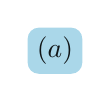
\begin{tikzpicture}[baseline=-0.5ex] \node [draw=none, fill=cyan!80!black, fill opacity=0.4, text opacity=0.9, rounded corners] (blah) {$(a)$}; \end{tikzpicture}
\quad \FPR(\pos_2, r) < \tprsymb &\rightarrow \FPR(\pos_1, r) < \FPR(\pos_2, r), \\

\begin{tikzpicture}[baseline=-0.5ex] \node [draw=none, fill=red!80!black, fill opacity=0.4, text opacity=0.9, rounded corners] (blah) {$(b)$}; \end{tikzpicture}
\quad \FPR(\pos_2, r) > \tprsymb &\rightarrow \FPR(\pos_1, r) > \FPR(\pos_2, r).
\end{align*}
(a) corresponds to a ranking and cutoff that is better than random (i.e. $\TPR(\pos,r) > \FPR(\pos,r)$) whereas (b) corresponds to a ranking and cutoff that is worse than random.

\begin{figure}[!h]
  \centering
  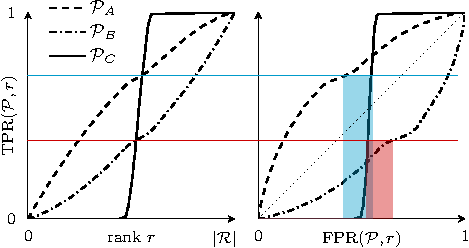
\includegraphics[width=0.6\textwidth]{lemma_size_fpr.pdf}
  \caption[]{Illustration of Lemma~\ref*{lemma-size-fpr}, with $\pos_A \subset \overall$, $\pos_B \subset \overall$, $\pos_C \subset \overall$, 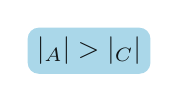
\begin{tikzpicture}[baseline=-0.5ex] \node [draw=none, fill=cyan!80!black, fill opacity=0.4, text opacity=0.9, rounded corners] (blah) {$|\pos_A| > |\pos_C|$}; \end{tikzpicture} and 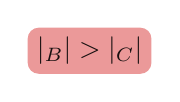
\begin{tikzpicture}[baseline=-0.5ex] \node [draw=none, fill=red!80!black, fill opacity=0.4, text opacity=0.9, rounded corners] (blah) {$|\pos_B| > |\pos_C|$}; \end{tikzpicture}. If two sets of positives $\pos_1$ and $\pos_2$ achieve a given TPR at the same rank $r$, e.g. $\TPR(\pos_1,r)=\TPR(\pos_2,r)$ and $|\pos_1| > |\pos_2|$ then $\FPR(\pos_1,r) < \FPR(\pos_2,r)$ if $\FPR(\pos_2,r) < \TPR(\pos_2,r)$ and otherwise $\FPR(\pos_1,r) > \FPR(\pos_2,r)$.} 
  \label{fig:lemma-size-fpr}
\end{figure}

\textbf{Proof}: take the derivative of FPR to $|\pos|$ while fixing $\ranksymb$, based on Equation~\eqref{tpr-fpr}:
\begin{align}
\frac{d\FPR(\pos, \ranksymb)}{d|\pos|} &= \frac{\ranksymb-\tprsymb\cdot|\overall|}{(|\overall|-|\pos|)^2}, \nonumber \\
&= \frac{\ranksymb-\tprsymb\cdot|\pos| - \tprsymb \cdot|\overall-\pos|}{(|\overall|-|\pos|)^2}. \label{FPR_ifv_gamma}
\end{align}
$r-\tprsymb\cdot|\pos|$ is the number of negatives in the top ranking (false positives) and $\tprsymb\cdot|\overall - \pos|$ is the number of false positives at $\FPR=\tprsymb$. The derivative is negative if the $\FPR$ is below $\tprsymb$ and vice versa, therefore if the ranking is better than random ($\TPR = \tprsymb > \FPR$), increasing $|\pos|$ leads to a lower $\FPR$ at rank $\ranksymb$ and vice versa. \hfill $\blacksquare$
\end{lemma}

Lemma~\ref*{lemma-size-fpr} has a large practical impact. If the ranking of $\knownpos$ is better than random, then over and under estimating $\hat{\pfrac}$ is useful to obtain a (loose) upper/lower bound on performance curves, respectively. In other words, given bounds or a CI on $\pfrac$, that is $\hat{\pfrac}_{lo} \leq \pfrac \leq \hat{\pfrac}_{up}$, we can use $\hat{\pfrac}_{lo}$ and $\hat{\pfrac}_{up}$ to estimate a lower and upper bound on the true ROC or PR curve. Bounds computed based on a CI for $\pfrac$ constitute a CI for the performance metric (at the same confidence level), assuming the rank CDF of $\latentpos$ is contained by the confidence band on the rank CDF. Tighter bounds on $\pfrac$ translate directly to tighter bounds on performance estimates. Finally, treating the full unlabeled set as negative results underestimates performance, since $\hat{\pfrac}=0 < \pfrac$. The effect of varying $\hat{\pfrac}$ is shown in Figure~\ref{fig:roc-ifv-beta}.

\begin{figure}[!h]
	\centering
	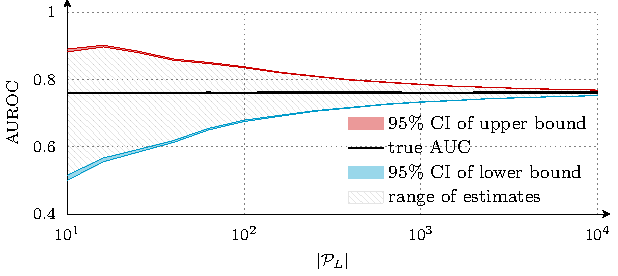
\includegraphics[width=0.8\textwidth]{convergence.pdf}
	\vfill	
	\caption{The effect of $|\knownpos|$ on estimated AUC. Based on $|\unlabeled| = 100,000$, $\knownneg=\emptyset$ and $\hat{\pfrac}=\pfrac=0.2$. Bounds on rank CDF were obtained via bootstrap. The depicted confidence intervals are based on 200 repeated experiments.}
	\label{fig:convergence}
\end{figure}
\begin{figure}[!h]
	\centering
	\centering
	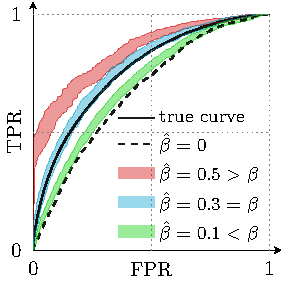
\includegraphics[width=0.4\textwidth]{roc_ifv_beta.pdf}
	\vfill
	\caption{The effect of $\hat{\pfrac}$ on estimated ROC curves, based on 2,000 known positives, 100,000 unlabeled instances and $\pfrac=0.3$.}
	\label{fig:roc-ifv-beta}
\end{figure}

%Given the relationship between ROC and PR curves as explained in Section~\ref{roc-pr}, the pattern in Figure~\ref{fig:roc-ifv-beta} applies to PR curves too: overestimating $\hat{\pfrac}$ results in overly optimistic bounds (can yield a loose upper bound) while underestimating $\hat{\pfrac}$ results in pessimistic bounds (can yield a loose lower bound).

\subsection{Model selection}
Often evaluation metrics are used to select the best model from a set of candidates. If model A's ROC (PR) curve dominates model B's ROC (PR) curve, then for all $\pfrac$ model A is better than model B (leaving aside significance testing). However, in most cases one model does not dominate another model and there exists a point where the two curves cross. Surprisingly, the ordering in terms of both AUROC and AUPR are dependent on $\hat{\pfrac}$ when this happens. This means that the ordering of models according to these metrics can switch when $\hat{\pfrac}$ changes. Figure~\ref{rocauc-switch} depicts an example that illustrates this. This demonstrates that $\hat{\pfrac}$ can play a crucial role in model selection. In the likely event that the curves cross, it is important to look at the range of possible values for $\hat{\pfrac}$ that represent different operating conditions when selecting among different models.

%there is strict dominance ordering of the models, that is, for a given FPR, model A's TPR is always greater than or equal to model B's TPR, then 


A more formal explanation of why this occurs can be made based on partial derivatives of each entry of the partial contingency table and TPR, FPR and precision based on unlabeled instances to $\hat{\pfrac}$:\footnote{We made some simplifications, the details are described in Appendix~\ref*{partial}.}
\begin{align}
\frac{\partial \TPR_U^r}{\partial \hat{\pfrac}} &= 0,\\
\frac{\partial \FPR_U^r}{\partial \hat{\pfrac}} &= \frac{|\topfun(\unlabeled, r)| - \mathcal{T}(r) \cdot |\unlabeled|}{(1-\hat{\pfrac})^2}, \label{eq:partials} \\
\frac{\partial \PREC_U^r}{\partial \hat{\pfrac}} &= \frac{\mathcal{T}(r)\cdot|\unlabeled|}{|\topfun(\unlabeled,r)|} \geq 0.
\end{align}
The partial derivative of TPR is exactly 0 because our approach is based on rank CDFs (that is TPR at each rank). Interestingly, the partial derivatives of FPR and precision to $\hat{\pfrac}$ are dependent on the value of the rank CDF $\mathcal{T}(r)$ that is being used to infer surrogate positives. Since $\TPR$ is not a function of $\hat{\pfrac}$ and the partial derivatives of $\FPR$/precision to $\hat{\pfrac}$ are functions of $\mathcal{T}(r)$, distinct segments of an ROC/PR curve are moved differently when $\hat{\pfrac}$ changes, inducing a non-uniform scaling of AUC across the TPR range. Such scaling potentially changes the ordering of models based on AUC. 
% property. 

%Model selection aims to identify the best model from a set of candidates and involves a series of pair-wise comparisons of classifiers $A$ and $B$ to decide which is best, based on empirical measurements of some metric such as AUROC. Each model is characterized by the rank CDF of known positives based on that model's predictions, that is $\mathcal{T}_A(r)$ and $\mathcal{T}_B(r)$. The rank CDF is used to infer surrogate positives $\surrpos$ from the unlabeled set $\unlabeled$ in order to estimate the performance metric of interest. 

%Since $\TPR$ is not a function of $\hat{\pfrac}$ and the partial derivative of $\FPR$ to $\hat{\pfrac}$ is a function of $\mathcal{T}(r)$, distinct segments of an ROC curve are moved differently when $\hat{\pfrac}$ changes, inducing a non-uniform scaling of AUC across the TPR range. A direct result of this observation is that the best model in terms of AUROC is contingent on $\hat{\pfrac}$, i.e. it is possible for a model to become better than another in terms of AUROC when $\hat{\pfrac}$ changes, given that the rank distributions $\mathcal{T}_A(r)$ and $\mathcal{T}_B(r)$ of both models cross. The sensitivity of AUROC to $\hat{\pfrac}$ depends on the shape of the curve.  The same reasoning applies to PR curves, since the partial derivative of precision to $\hat{\pfrac}$ is also a function of $\mathcal{T}(r)$. This proves that good estimates of $\hat{\pfrac}$ are necessary for correct model selection (and hence, using $\hat{\pfrac}=0$ to perform model selection is suboptimal). Figure~\ref{rocauc-switch} depicts an example illustrating this property. 
\begin{figure}[!h]
\centering
  \begin{minipage}[c]{0.45\textwidth}
  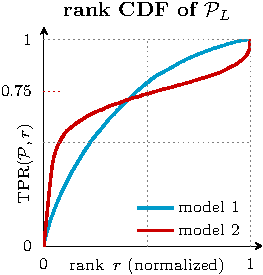
\includegraphics[width=\textwidth]{switch_cdf.pdf}
  \end{minipage}\hfill
  \begin{minipage}[c]{0.45\textwidth}
  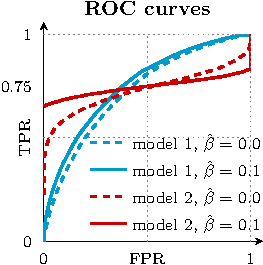
\includegraphics[width=\textwidth]{switch_roc.pdf}
  \end{minipage}
\caption[]{The effect of $\hat{\pfrac}$ on ROC curves. Setup: $|\unlabeled|=45,000$, $|\knownpos|=5,000$. \\%Model 2 wins for $\hat{\pfrac}=0$, but model 1 wins for $\hat{\pfrac}=0.1$. %The curve for model 2 is independent of $\hat{\pfrac}$. 

Corresponding AUROC (best in bold): 
{\centering
\begin{tabular}{ccc}
\toprule
estimated $\hat{\pfrac}$ 	& model 1 	& model 2 \\
\midrule
0.0		& $72.5\%$		& $\mathbf{73.2\%}$ \\
0.1		& $\mathbf{75.5\%}$	& $74.7\%$ \\
\bottomrule
\end{tabular}}
}\label{rocauc-switch}
\end{figure}


\subsection{Empirical quality of the estimates} \label{empirical}
We illustrate the quality of our estimated bounds on ROC and PR curves using a model trained in a PU learning setting [BLINDED for review] on the \covtype data set \citep{Blackard00covtype}. The model was evaluated on a fully labeled test set of $20,000$ positive and $20,000$ negative examples. To estimate performance, we randomly selected $5\%$ of positive examples to serve as our labeled set and treated all other examples as unlabeled, which yields $|\knownpos|=1,000$, $|\unlabeled| = 39,000$ and $\pfrac\approx49\%$. We present ROC and PR curves with bounds for $\hat{\pfrac}=\pfrac$, $\hat{\pfrac}=0$, and a confidence interval $\hat{\pfrac}_{lo} = 0.8\pfrac \leq \hat{\pfrac} \leq \hat{\pfrac}_{up} = 1.2\pfrac$. Finally, as we have the ground truth, we present true curves as a reference.\footnote{Python code to reproduce all results (and modify the configuration) is available as supplementary material.}

Figure~\ref{fig:results-covtype} presents  the rank CDF and estimated bounds on ROC and PR curves. Figure~\ref{fig:results-covtype-cdf} shows the true rank CDF of $\latentpos$ along with an estimated $95\%$ CI on the rank CDF using the $\knownpos$ via a standard bootstrap approach with $2,000$ resamples. In this case, the CI contains the true rank CDF of latent positives.\footnote{The rank CDF of $\latentpos$ is unknown in practice, but assumed to be comparable to the rank CDF of $\knownpos$.} Figures~\ref{fig:results-covtype-roc} and~\ref{fig:results-covtype-pr} show that the bounds closely approximate the true performance curves. The estimated bounds are wider in PR space than in ROC space, particularly at low recall. Note that estimated PR curves are sensitive to the estimation error in $\hat{\pfrac}$, as precision is directly affected by class balance, limiting their usefulness if only a rough estimate of $\pfrac$ is available.

%Figure~\ref{fig:results-covtype} presents the rank CDF and estimated bounds on ROC and PR curves. Figure~\ref{fig:results-covtype-cdf} shows the true rank CDF along with an estimated $95\%$ CI on the rank CDF using the $\knownpos$ via a standard bootstrap approach with $2,000$ resamples. In this case, the CI contains the true rank CDF of latent positives (which is unknown in practice). Hence, the true ROC and PR curves assuming all labels are know are guaranteed to be between the bounds estimated using the partial labeled data, assuming that $\hat{\pfrac}_{lo} \leq \pfrac \leq \hat{\pfrac}_{up}$. This can be confirmed in Figures~\ref{fig:results-covtype-roc} and~\ref{fig:results-covtype-pr}.

%The bounds closely approximate the true performance curves, depending on the quality of $\hat{\pfrac}$ and the width of the CI on rank CDF. The estimated bounds are wider in PR space than in ROC space, particularly at low recall (Figure~\ref{fig:results-covtype-pr} and~\ref{fig:results-covtype-roc}, respectively). Additionally, it must be noted that estimated PR curves are very sensitive to the estimation error in $\hat{\pfrac}$, because precision is directly affected by class balance. As such, we recommend using ROC curves over PR curves when only a rough estimate of $\pfrac$ is available.



\begin{figure}%
\centering
\subfloat[Rank CDF.\label{fig:results-covtype-cdf}]{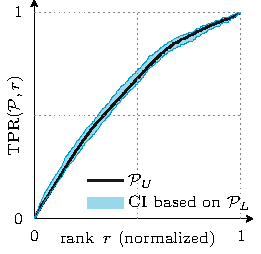
\includegraphics[width=0.31\textwidth]{covtype_cdf.pdf}}\hfill
\subfloat[ROC curves.\label{fig:results-covtype-roc}]{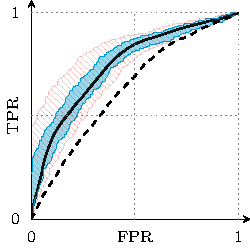
\includegraphics[width=0.31\textwidth]{covtype_roc.pdf}}\hfill
\subfloat[PR curves.\label{fig:results-covtype-pr}]{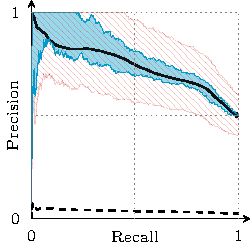
\includegraphics[width=0.31\textwidth]{covtype_pr.pdf}}\\
\caption[]{Results for \covtype showing rank CDF, ROC and PR curves, with $\pfrac\approx 49\%$.
Performance curve legend:  \newline
\begin{tikzpicture}[baseline=-0.5ex] \draw [color=black, thick] (0, 0) -- (0.5, 0); \end{tikzpicture} true curve, 
\begin{tikzpicture}[baseline=-0.5ex] \draw [color=black, thick, dashed] (0, 0) -- (0.5, 0); \end{tikzpicture} $\hat{\pfrac}=0$, 

\begin{tikzpicture}[baseline=-0.5ex] \draw [color=cyan!80!black, opacity=0.8] (0, -0.2) rectangle (0.7, 0.3); 
\fill [color=cyan!80!black, opacity=0.4] (0, -0.2) rectangle (0.7, 0.3); \end{tikzpicture} $\hat{\pfrac}=\pfrac$ and 

\begin{tikzpicture}[baseline=-0.5ex] \draw [color=red!80!black, opacity=0.2, pattern=north west lines, pattern color=red!80!black] (0, -0.2) rectangle (0.7, 0.3); \end{tikzpicture} $0.8\pfrac \leq \hat{\pfrac} \leq 1.2\pfrac$.}
\label{fig:results-covtype}
\end{figure}

\ifx
\begin{figure}[h]
\centering
\subfigure[Rank CDF.\label{fig:results-covtype-cdf}]{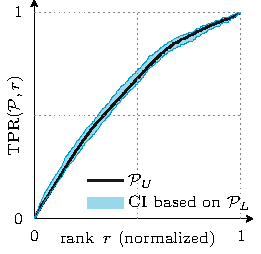
\includegraphics[width=0.25\textwidth]{covtype_cdf.pdf}}\qquad
\subfigure[ROC curves.\label{fig:results-covtype-roc}]{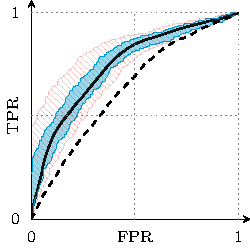
\includegraphics[width=0.25\textwidth]{covtype_roc.pdf}}\qquad
\subfigure[PR curves.\label{fig:results-covtype-pr}]{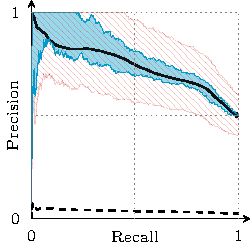
\includegraphics[width=0.25\textwidth]{covtype_pr.pdf}}
\addtolength{\abovecaptionskip}{-3mm}
%\subfigure[Rank CDF for \sensit.]{\includegraphics[width=0.29\textwidth]{cdf_sensit_2_semi_resvm.pdf}}\qquad
%\subfigure[ROC curves for \sensit.]{\includegraphics[width=0.29\textwidth]{roc_sensit_2_semi_resvm.pdf}}\qquad
%\subfigure[PR curves for \sensit.]{\includegraphics[width=0.29\textwidth]{pr_sensit_2_semi_resvm.pdf}}
%\caption{Results for \covtype and \sensit showing rank CDF, ROC and PR curves (left to right).}
\caption[]{Results for \covtype showing rank CDF, ROC and PR curves, with $\pfrac\approx 49\%$. \newline
Performance curve legend: 
\begin{tikzpicture}[baseline=-0.5ex] \draw [color=black, thick] (0, 0) -- (0.5, 0); \end{tikzpicture} true curve, 
\begin{tikzpicture}[baseline=-0.5ex] \draw [color=black, thick, dashed] (0, 0) -- (0.5, 0); \end{tikzpicture} $\hat{\pfrac}=0$, 

\begin{tikzpicture}[baseline=-0.5ex] \draw [color=cyan!80!black, opacity=0.8] (0, -0.2) rectangle (0.7, 0.3); 
\fill [color=cyan!80!black, opacity=0.4] (0, -0.2) rectangle (0.7, 0.3); \end{tikzpicture} $\hat{\pfrac}=\pfrac$ and 

\begin{tikzpicture}[baseline=-0.5ex] \draw [color=red!80!black, opacity=0.2, pattern=north west lines, pattern color=red!80!black] (0, -0.2) rectangle (0.7, 0.3); \end{tikzpicture} $0.8\pfrac \leq \hat{\pfrac} \leq 1.2\pfrac$.}
\label{fig:results-covtype}
\addtolength{\abovecaptionskip}{3mm}
\end{figure}
\fi


%positive labels (chosen at random), ignored all negative labels along with $95\%$ of positive labels (chosen at random), which yields $|\knownpos|=1,000$, $|\unlabeled| = 39,000$ and $\pfrac\approx49\%$. We have computed bounds on the ROC and PR curves based on treating $\unlabeled$ as negative (i.e., $\hat{\pfrac}=0$), the right amount of latent positives (i.e., $\hat{\pfrac}=\pfrac$) and a confidence interval ($\hat{\pfrac}_{lo} = 0.8\pfrac \leq \hat{\pfrac} \leq \hat{\pfrac}_{up} = 1.2\pfrac$). Having all test labels enabled us to compute true performance curves as a reference. \footnote{Python code to reproduce all results (and modify the configuration) is available as supplementary material.}

 %(consisting of $20,000$ positives and negatives). Having all test labels enabled us to compute true performance curves as a reference. 



%To illustrate our approach, we estimated bounds on ROC and PR curves and compared these to the ground truth. We used rankings and corresponding true labels of simulations done by BLINDED, in which classifiers were tuned and trained in a PU learning context on the \covtype data set \citep{Blackard00covtype} and tested on an independent, fully labeled test set (consisting of $20,000$ positives and negatives). Having all test labels enabled us to compute true performance curves as a reference. 

%To produce our estimations, we ignored all negative labels along with $95\%$ of positive labels (chosen at random), which yields $|\knownpos|=1,000$, $|\unlabeled| = 39,000$ and $\pfrac\approx49\%$. We have computed bounds on the ROC and PR curves based on treating $\unlabeled$ as negative (i.e., $\hat{\pfrac}=0$), the right amount of latent positives (i.e., $\hat{\pfrac}=\pfrac$) and a confidence interval ($\hat{\pfrac}_{lo} = 0.8\pfrac \leq \hat{\pfrac} \leq \hat{\pfrac}_{up} = 1.2\pfrac$). Python code to reproduce all results (and modify the configuration) is available as supplementary material.

%Figure~\ref{fig:results-covtype} shows the rank CDF and estimated bounds on ROC and PR curves. We estimated a $95\%$ CI on the rank CDF of $\knownpos$ via a standard bootstrap approach, using $2,000$ resamples. As the confidence band on rank CDF contains the true rank CDF of latent positives (which is unknown in practice), the true ROC and PR curves (based on $\bothpos$) are guaranteed to be between the respective bounds (based on $\bothposapprox$), given $\hat{\pfrac}=\pfrac$ or $\hat{\pfrac}_{lo} \leq \pfrac \leq \hat{\pfrac}_{up}$, as is confirmed by the results in Figure~\ref{fig:results-covtype}.

%The bounds closely approximate the true performance curves, depending on the quality of $\hat{\pfrac}$. The estimated bounds are wider in PR space than in ROC space, particularly at low recall (Figure~\ref{fig:results-covtype-pr} and~\ref{fig:results-covtype-roc}, respectively). Additionally, it must be noted that estimated PR curves are very sensitive to the estimation error in $\hat{\pfrac}$, because precision is directly affected by class balance. As such, we recommend using ROC curves over PR curves when only a rough estimate of $\pfrac$ is available.


\subsection{Relative importance of known negatives compared to known positives}
As our approach can incorporate known negatives, a natural question is how their presence influences the estimates. In practice, a test set is of fixed size, so known negatives essentially reduce the size of the unlabeled subset, which in turn reduces the number of degrees of freedom in assigning surrogate positives. Using the same setup as in Subsection~\ref{empirical}, we varied the proportion of known positives and negatives and found known negatives provide some benefit, though this is small in practice. However, our approach can also be reversed given a large amount of negatives, that is flip known class labels, use $\bar{\pfrac}=1-\pfrac$ and adjust the resulting contingency tables accordingly, which can improve performance bounds. The benefits of known negatives are further discussed in Appendix~\ref*{knownneg}.




%benefit does their presence

%n

%nown negatives can b incorporated in our approach as described in Section~\ref{contingency}. Given a fixed ranking $\overall$, having known negatives essentially reduces the size of the unlabeled subset $\unlabeled$, which in turn reduces the number of degrees of freedom in assigning surrogate positives. As such, known negatives provide some benefit, though this is small in practice (see Appendix~\ref*{knownneg} for an example).

%However, when the number of known negatives is large enough our approach can be reversed, that is flip known class labels, use $\pfrac$ to $\bar{\pfrac}=1-\pfrac$ and adjust the resulting contingency tables accordingly. Hence, bounds can be computed based primarily on known positives $\knownpos$ \emph{or} known negatives $\knownneg$. The width of the bounds depends on the combination of $|\knownpos|$ (or $|\knownneg|$) and $\pfrac$ (or $\bar{\pfrac}$) in a nontrivial way: depending on $\pfrac$, it is possible to obtain wider bounds based on known negatives, even if $|\knownneg| > |\knownpos|$ (or vice versa). In practice, we can estimate metrics based on $\knownpos$ and $\knownneg$ separately and then use whichever yields the tightest bounds. More information is included in Appendix~\ref*{knownneg}.

\section{Conclusion}
We presented an approach to construct contingency tables corresponding to a lower and upper bound on FPR using only partially labeled, which enables computing many commonly used performance metrics in a semi-supervised setting. Our approach relies on knowing the fraction of latent positives in the unlabeled data, and we discussed its effect on determing the bounds and model selection. We have seen that our approach can yield good estimates in practice.  

%at a given rank based on a confidence interval on the rank CDF of (known) positives. Via these estimated contingency tables many commonly used performance metrics become available in a semi-supervised setting. We have shown that the bounds enable proper model evaluation, though model selection based on AUROC requires good estimates of the fraction of latent positives in the unlabeled set ($\pfrac$). Poor estimates of $\pfrac$ may invalidate the bounds and hamper model selection.

%Our approach was used to compute bounds on ROC and PR curves in a realistic experiment, the quality of which is limited only by the quality of estimated confidence intervals on the CDF of ranks of positives and the estimated fraction of latent positives $\hat{\pfrac}$. Due to the sensitivity of the bounds in PR space to $\hat{\pfrac}$, we recommend using ROC curves for model evaluation in a partial labeling context. 

%\input{properties.tex}
%\newcommand{\covtype}{\texttt{covtype}\xspace}
\newcommand{\sensit}{\texttt{sensit}\xspace}

% no longer in use
\newcommand{\resultcurves}[2]{
\begin{figure}[!h]
\centering
\subfigure[\covtype.]{\includegraphics[width=0.22\textwidth]{#1_covtype_pu_resvm.pdf}}\qquad
\subfigure[\sensit.]{\includegraphics[width=0.22\textwidth]{#1_sensit_2_semi_resvm.pdf}}\\
\caption{#2}
\label{fig:results-#1}
\end{figure}
}

\newcommand{\resultcurvesnew}[2]{
\begin{figure}[!h]
\centering
%\subfigure[Rank CDF for \covtype.]{\includegraphics[width=0.2\textwidth]{cdf_covtype_pu_resvm.pdf}}\qquad
%\subfigure[ROC curves for \covtype.]{\includegraphics[width=0.2\textwidth]{roc_covtype_pu_resvm.pdf}}\qquad
%\subfigure[PR curves for \covtype.]{\includegraphics[width=0.2\textwidth]{pr_covtype_pu_resvm.pdf}}
\subfigure[Rank CDF for \covtype.]{\includegraphics[width=0.2\textwidth]{#1_cdf.pdf}}\qquad
\subfigure[ROC curves for \covtype.]{\includegraphics[width=0.2\textwidth]{#1_roc.pdf}}\qquad
\subfigure[PR curves for \covtype.]{\includegraphics[width=0.2\textwidth]{#1_pr.pdf}}
\caption{#2}
\label{fig:results-#1}
\end{figure}
}

\section{Results and discussion} \label{results}
%To demonstrate the applicability and robustness of our approach, we show the resulting estimates of ROC and PR curves on two public data sets in a PU learning setting and compare our estimates to the truth.\footnote{Python scripts and data to reproduce the results are provided in the supplementary material. We will publicly release the code after acceptance.}
%
%We used rankings and corresponding true labels of simulations done by BLINDED, in which classifiers were tuned and trained in a PU learning context and tested on an independent, fully labeled test set. Since all test labels are available, this enables us to compute the true curves as a reference. We used the rankings produced by the approach introduced in BLINDED on the \covtype and \sensit data sets \citep{Blackard00covtype, duarte2004vehicle}. The \covtype test set consists of $20,000$/$20,000$ positives/negatives and the \sensit test set consists of $5,250$/$14,455$ positives/negatives.
%
%In our estimations, we discarded all negative labels and $90\%$ of positive labels (at random). This setup yields $|\knownpos|=2,000$ and $\pfrac\approx47\%$ for \covtype and $|\knownpos|=525$ and $\pfrac\approx24\%$ for \sensit. We always used $\hat{\pfrac}=\pfrac$. We constructed $95\%$ confidence intervals on the rank CDF of $\knownpos$ via a bootstrap approach, using $2,000$ resamples.

To illustrate our approach, we estimated bounds on ROC and PR curves and compared these to the ground truth. We used rankings and corresponding true labels of simulations done by BLINDED, in which classifiers were tuned and trained in a PU learning context on the \covtype data set \citep{Blackard00covtype} and tested on an independent, fully labeled test set (consisting of $20,000$ positives and negatives). Having all test labels enabled us to compute true performance curves as a reference. 

To produce our estimations, we ignored all negative labels along with $95\%$ of positive labels (chosen at random), which yields $|\knownpos|=1,000$, $|\unlabeled| = 39,000$ and $\pfrac\approx49\%$. We have computed bounds on the ROC and PR curves based on treating $\unlabeled$ as negative (i.e., $\hat{\pfrac}=0$), the right amount of latent positives (i.e., $\hat{\pfrac}=\pfrac$) and a confidence interval ($\hat{\pfrac}_{lo} = 0.8\pfrac \leq \hat{\pfrac} \leq \hat{\pfrac}_{up} = 1.2\pfrac$). Python code to reproduce all results (and modify the configuration) is available as supplementary material.

The rank CDF and estimated bounds on ROC and PR curves are shown in Figure~\ref{fig:results-covtype}. We estimated a $95\%$ CI on the rank CDF of $\knownpos$ via a standard bootstrap approach, using $2,000$ resamples. As the confidence band on rank CDF contains the true rank CDF of latent positives (which is unknown in practice), the true ROC and PR curves (based on $\bothpos$) are guaranteed to be between the respective bounds (based on $\bothposapprox$), given $\hat{\pfrac}=\pfrac$ or $\hat{\pfrac}_{lo} \leq \pfrac \leq \hat{\pfrac}_{up}$, as is confirmed by the results in Figure~\ref{fig:results-covtype}.

The bounds closely approximate the true performance curves, depending on the quality of $\hat{\pfrac}$. The estimated bounds are wider in PR space than in ROC space, particularly at low recall (Figure~\ref{fig:results-covtype-pr} and~\ref{fig:results-covtype-roc}, respectively). Additionally, it must be noted that estimated PR curves are very sensitive to the estimation error in $\hat{\pfrac}$, because precision is directly affected by class balance. As such, we recommend using ROC curves over PR curves when only a rough estimate of $\pfrac$ is available.


%\resultcurves{pr}{Precision-Recall curves.}

\begin{figure}[!h]
\centering
\subfigure[Rank CDF.\label{fig:results-covtype-cdf}]{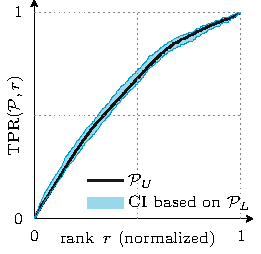
\includegraphics[width=0.25\textwidth]{covtype_cdf.pdf}}\qquad
\subfigure[ROC curves.\label{fig:results-covtype-roc}]{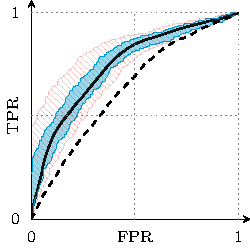
\includegraphics[width=0.25\textwidth]{covtype_roc.pdf}}\qquad
\subfigure[PR curves.\label{fig:results-covtype-pr}]{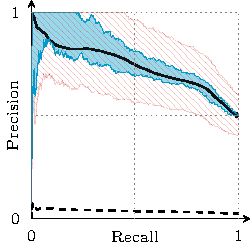
\includegraphics[width=0.25\textwidth]{covtype_pr.pdf}}
\addtolength{\abovecaptionskip}{-3mm}
%\subfigure[Rank CDF for \sensit.]{\includegraphics[width=0.29\textwidth]{cdf_sensit_2_semi_resvm.pdf}}\qquad
%\subfigure[ROC curves for \sensit.]{\includegraphics[width=0.29\textwidth]{roc_sensit_2_semi_resvm.pdf}}\qquad
%\subfigure[PR curves for \sensit.]{\includegraphics[width=0.29\textwidth]{pr_sensit_2_semi_resvm.pdf}}
%\caption{Results for \covtype and \sensit showing rank CDF, ROC and PR curves (left to right).}
\caption[]{Results for \covtype showing rank CDF, ROC and PR curves, with $\pfrac\approx 49\%$. \newline
Performance curve legend: 
\begin{tikzpicture}[baseline=-0.5ex] \draw [color=black, thick] (0, 0) -- (0.5, 0); \end{tikzpicture} true curve, 
\begin{tikzpicture}[baseline=-0.5ex] \draw [color=black, thick, dashed] (0, 0) -- (0.5, 0); \end{tikzpicture} $\hat{\pfrac}=0$, 

\begin{tikzpicture}[baseline=-0.5ex] \draw [color=cyan!80!black, opacity=0.8] (0, -0.2) rectangle (0.7, 0.3); 
\fill [color=cyan!80!black, opacity=0.4] (0, -0.2) rectangle (0.7, 0.3); \end{tikzpicture} $\hat{\pfrac}=\pfrac$ and 

\begin{tikzpicture}[baseline=-0.5ex] \draw [color=red!80!black, opacity=0.2, pattern=north west lines, pattern color=red!80!black] (0, -0.2) rectangle (0.7, 0.3); \end{tikzpicture} $0.8\pfrac \leq \hat{\pfrac} \leq 1.2\pfrac$.}
\label{fig:results-covtype}
\addtolength{\abovecaptionskip}{3mm}
\end{figure}

%%%%%%%%%%%%%%%%%%%%%%%%%%%%%%%%%%%%%%%%%%%%%%%%%%
%%%%%%%%%%%%%%%%%%%%%%%%%%%%%%%%%%%%%%%%%%%%%%%%%%
%
% 	Conclusion
%
%%%%%%%%%%%%%%%%%%%%%%%%%%%%%%%%%%%%%%%%%%%%%%%%%%
%%%%%%%%%%%%%%%%%%%%%%%%%%%%%%%%%%%%%%%%%%%%%%%%%%

\section{Conclusion}
We presented an approach to compute contingency tables corresponding to a lower and upper bound on FPR at a given rank based on a confidence interval on the rank CDF of (known) positives. Via these estimated contingency tables many commonly used performance metrics become available in a semi-supervised setting. We have shown that the bounds enable proper model evaluation, though model selection based on AUROC requires good estimates of the fraction of latent positives in the unlabeled set ($\pfrac$). Poor estimates of $\pfrac$ may invalidate the bounds and hamper model selection.

Our approach was used to compute bounds on ROC and PR curves in a realistic experiment, the quality of which is limited only by the quality of estimated confidence intervals on the CDF of ranks of positives and the estimated fraction of latent positives $\hat{\pfrac}$. Due to the sensitivity of the bounds in PR space to $\hat{\pfrac}$, we recommend using ROC curves for model evaluation in a partial labeling context. % unless $\hat{\pfrac}$ is known to be good estimate. %The proposed bounds enable thorough model assessment in a semi-supervised setting.% and hence address an important practical problem.


% Acknowledgements should only appear in the accepted version. 
\section*{Acknowledgments} 
Will be inserted after review.
%STADIUS members are supported by Flemish Government: FWO: projects:  G.0871.12N (Neural circuits), IWT: TBM-Logic Insulin(100793), TBM Rectal Cancer(100783), TBM IETA(130256); PhD grant \#111065, Industrial Research fund (IOF): IOF Fellowship 13-0260; iMinds Medical Information Technologies SBO 2015, ICON projects (MSIpad, MyHealthData)
%VLK Stichting E. van der Schueren: rectal cancer; Federal Government: FOD: Cancer Plan 2012-2015 KPC-29-023 (prostate); COST: Action: BM1104: Mass Spectrometry Imaging. Jesse Davis is partially supported by the Research Fund KU Leuven (OT/11/051), EU FP7 Marie Curie Career Integration Grant (\#294068) and FWO-Vlaanderen (G.0356.12).
\newpage
\bibliography{bibliography}
\bibliographystyle{unsrt}

\newpage
\section*{Supplementary material for ``\emph{Assessing Binary Classifiers Using Only Positive and Unlabeled Data}"}
\appendix
\section{Effect of $\hat{\pfrac}$ on contingency table entries and common performance metrics} \label{partial}
To study the effect of imprecise estimates of $\pfrac$, we start by computing partial derivatives of each entry of the partial contingency table based on unlabeled instances to $\hat{\pfrac}$ (see Section~\ref{contingency}). Subsequently, we will compute partial derivatives of TPR, FPR and precision to $\hat{\pfrac}$ to describe the effect of estimating $\pfrac$ on (area under) ROC and PR curves.

For ease of notation, we base all subsequent calculations on $\tilde{\theta} = \hat{\pfrac} \mathcal{T}(r) \cdot |\unlabeled| \approx \theta$ which ignores the discrete effect of rounding in the real definition of $\theta$ (Eq.~\ref{theta}). We additionally assume it is possible to assign the desired amount $\tilde{\theta}$ of surrogate positives in $\topfun(\unlabeled, r)$, which holds for ranks $r$ that are not too close to the top or bottom of $\overall$, given reasonable values of $\hat{\pfrac}$ and CDF bounds $\mathcal{T}(r)$.\footnote{$\mathcal{T}(r)$ represents a bound on rank CDF, that is either $\mathcal{T}_{lb}(r)$ or $\mathcal{T}_{ub}(r)$ as used in the manuscript.} If this does not hold, that is when there is clipping in Eq.~\ref{eq:surrpos-conditions}, then (small) changes in $\hat{\pfrac}$ do not affect $\TP_U^r$ and hence the partial derivatives of \emph{all} entries in the contingency table to $\hat{\pfrac}$ are effectively 0.

Given these simplifications, the partial contingency table based on unlabeled instances becomes:
\begin{align*}
\TP_U^r &= \tilde{\theta} = \hat{\pfrac}\mathcal{T}(r) \cdot |\unlabeled| \\
\FN_U^r &= |\surrpos| - \TP_U^r = \hat{\pfrac}\cdot |\unlabeled| - \hat{\pfrac}\mathcal{T}(r) \cdot |\unlabeled| = \hat{\pfrac} \big(1-\mathcal{T}(r)\big) \cdot|\unlabeled| \nonumber \\
\FP_U^r &= |\topfun(\unlabeled, r)| - \TP_U^r = |\topfun(\unlabeled, r)| - \hat{\pfrac}\mathcal{T}(r) \cdot |\unlabeled|, \nonumber \\
\TN_U^r &= |\unlabeled| - |\surrpos| - \FP_U^r = |\unlabeled| - \hat{\pfrac}\cdot|\unlabeled| - |\topfun(\unlabeled, r)| + \hat{\pfrac}\mathcal{T}(r) \cdot |\unlabeled|, \\
	&= \big(1-\hat{\pfrac} + \hat{\pfrac}\mathcal{T}(r)\big) \cdot |\unlabeled| - |\topfun(\unlabeled, r)|.
\end{align*}
The partial derivatives of each entry of the partial contingency table then become:
\begin{align*}
\frac{\partial \TP_U^r}{\partial \hat{\pfrac}} &= \mathcal{T}(r) \cdot |\unlabeled| \geq 0, & &\frac{\partial \FP_U^r}{\partial \hat{\pfrac}} = -\mathcal{T}(r) \cdot |\unlabeled| \leq 0, \\
\frac{\partial \FN_U^r}{\partial \hat{\pfrac}} &= \big(1 -\mathcal{T}(r)\big) \cdot |\unlabeled| \geq 0, & &\frac{\partial \TN_U^r}{\partial \hat{\pfrac}} = \big(\mathcal{T}(r)-1\big) \cdot |\unlabeled| \leq 0.
\end{align*}

Partial derivatives for TPR, TPR and precision are a little more involved:
\begin{align}
\frac{\partial \TPR_U^r}{\partial \hat{\pfrac}} &= \frac{\frac{\partial \TP_U^r}{\partial \hat{\pfrac}} |\surrpos| - \TP_U^r \frac{\partial |\surrpos|}{\partial \hat{\pfrac}}}{|\surrpos|^2} 
= \frac{\mathcal{T}(r)\hat{\pfrac}\cdot|\unlabeled|^2-\mathcal{T}(r)\hat{\pfrac} |\unlabeled|^2}{\hat{\pfrac}^2|\unlabeled|^2} \nonumber \\
&= \frac{\mathcal{T}(r)-\mathcal{T}(r)}{\hat{\pfrac}} = 0 \label{eq:dtpr} \\
\frac{\partial \FPR_U^r}{\partial \hat{\pfrac}} &= \frac{\frac{\partial \FP_U^r}{\partial \hat{\pfrac}} \cdot (|\unlabeled|-|\surrpos|) - \FP_U^r \frac{\partial (|\unlabeled|-|\surrpos|)}{\partial \hat{\pfrac}}}{(|\unlabeled|-|\surrpos|)^2} \nonumber \\
&= \frac{-\mathcal{T}(r) \cdot |\unlabeled| \cdot (|\unlabeled|-|\surrpos|)+\FP_U^r \cdot |\unlabeled|}{(|\unlabeled|-|\surrpos|)^2} \nonumber \\
&=\frac{-\mathcal{T}(r) (1-\hat{\pfrac}) \cdot |\unlabeled|^2 + \FP_U^r \cdot |\unlabeled|}{(1-\hat{\pfrac})^2 \cdot |\unlabeled|^2} \nonumber \\
&=\frac{-\mathcal{T}(r)}{1-\hat{\pfrac}} + \frac{(|\topfun(\unlabeled, r)|-\hat{\pfrac}\mathcal{T}(r) \cdot |\unlabeled|) \cdot |\unlabeled|}{(1-\hat{\pfrac})^2 \cdot |\unlabeled|^2}  \nonumber \\
%&=\frac{-\mathcal{T}(r)}{1-\hat{\pfrac}} - \frapfrac}\mathcal{T}(r)}{(1-\hat{\pfrac})^2} + \frac{|\topfun(\unlabeled, r)|}{(1-\hat{\pfrac})^2\cdot|\unlabeled|} 
&=\frac{-\mathcal{T}(r)}{(1-\hat{\pfrac})^2} + \frac{|\topfun(\unlabeled, r)|}{(1-\hat{\pfrac})^2\cdot|\unlabeled|} 
= \frac{|\topfun(\unlabeled, r)| - \mathcal{T}(r) \cdot |\unlabeled|}{(1-\hat{\pfrac})^2} \label{eq:dfpr} \\
%=\frac{-\mathcal{T}(r)}{(1-\hat{\pfrac})^2} + \frac{|\topfun(\unlabeled, r)|}{(1-\hat{\pfrac})^2\cdot|\unlabeled|} \nonumber \\
%&= \frac{|\topfun(\unlabeled, r)| - \mathcal{T}(r) \cdot |\unlabeled|}{(1-\hat{\pfrac})^2} \label{eq:dfpr} \\
\frac{\partial \PREC_U^r}{\partial \hat{\pfrac}} &= \frac{\frac{\partial \TP_U^r}{\partial \hat{\pfrac}} \cdot (\TP_U^r+\FP_U^r) - \TP_U^r \frac{\partial (\TP_U^r+\FP_U^r)}{\partial \hat{\pfrac}}}{(\TP_U^r+\FP_U^r)^2} \nonumber \\ 
&= \frac{\mathcal{T}(r)\cdot|\unlabeled|\cdot(\TP_U^r + \FP_U^r)}{(\TP_U^r + \FP_U^r)^2} \nonumber \\
&= \frac{\mathcal{T}(r)\cdot|\unlabeled|}{(\TP_U^r + \FP_U^r)} = \frac{\mathcal{T}(r)\cdot|\unlabeled|}{|\topfun(\unlabeled,r)|} \geq 0 \label{eq:dprec} 
\end{align}
%$\partial \FPR_U^r / \partial \hat{\pfrac}$ is particularly interesting: it is positive if the ranking is better than random, i.e. $\TPR(\surrpos, r) > \FPR(\surrpos, r)$ and negative when the ranking is worse than random, i.e. $\TPR(\surrpos, r) < \FPR(\surrpos, r)$. This was already shown previously in Lemma~\ref{lemma-size-fpr}. 

Both $\partial \FPR_U^r / \partial \hat{\pfrac}$ and $\partial \PREC_U^r / \partial \hat{\pfrac}$ are a function of $\mathcal{T}(r)$, while $\partial \FPR_U^r / \partial \hat{\pfrac} = 0$. This implies that the ordering of rankings in terms of area under the ROC curve can change when the estimate of $\pfrac$ changes, as proven by example in Figure~\ref{rocauc-switch}.


\section{The effect of the fraction of known positives, known negatives and $\hat{\pfrac}$} \label{knownneg}
Known negatives can be incorporated in our approach as described in Section~\ref{contingency}. Given a fixed ranking $\overall$, having known negatives essentially reduces the size of the unlabeled subset $\unlabeled$, which in turn reduces the number of degrees of freedom in assigning surrogate positives. As such, known negatives provide some benefit, though this is small in practice. Table~\ref{parameffects-posonly} illustrates the effect of increasing amounts of known positives and known negatives: known positives significantly tighten bounds on AUROC, while known negatives only do so marginally (cfr. bounds with $10\%$ known positives and $40/60/80\%$ known negatives).

\def\realauc{0.765}

\newcommand{\plotauc}[2]{
\begin{tikzpicture}[baseline=1ex]
    \begin{axis}[hide axis,clip=false,
%	xmin=0.71,xmax=0.84,xlabel={X},
%	ymin=-1,ymax=1,
%	x=20cm, y=0.8em,
	xmin=0.67,xmax=0.87,xlabel={X},
	ymin=-1,ymax=1,
	x=12cm, y=0.8em,
	]

\addplot[black, very thick, dashed] coordinates {(\realauc, -1) (\realauc, 1)};
\addplot[gray, thick, dashed] coordinates {(0.67, -1) (0.67, 1)};
\addplot[gray, thick, dashed] coordinates {(0.87, -1) (0.87, 1)};
%\addplot[gray, thick, dashed] coordinates {(0.71, -1) (0.71, 1)};
%\addplot[gray, thick, dashed] coordinates {(0.83, -1) (0.83, 1)};
\addplot[black, dotted] coordinates {(0.73, -1) (0.73, 1)};
\addplot[black, dotted] coordinates {(0.75, -1) (0.75, 1)};
\addplot[black, dotted] coordinates {(0.77, -1) (0.77, 1)};
\addplot[black, dotted] coordinates {(0.79, -1) (0.79, 1)};
\addplot[black, dotted] coordinates {(0.81, -1) (0.81, 1)};
\addplot[gray, dotted] coordinates {(0.71, -1) (0.71, 1)};
\addplot[gray, dotted] coordinates {(0.69, -1) (0.69, 1)};
\addplot[gray, dotted] coordinates {(0.83, -1) (0.83, 1)};
\addplot[gray, dotted] coordinates {(0.85, -1) (0.85, 1)};
\draw [color=cyan!80!black, opacity=0.8] (axis cs: #1, -0.7) rectangle (axis cs: #2, 0.6);
\fill [color=cyan!80!black, opacity=0.4, fill] (axis cs: #1, -0.7) rectangle (axis cs: #2, 0.6);
    \end{axis}
\end{tikzpicture}
}
\newcommand{\plotauccolor}[3]{
\begin{tikzpicture}[baseline=1ex]
    \begin{axis}[hide axis,clip=false,
	xmin=0.67,xmax=0.87,xlabel={X},
	ymin=-1,ymax=1,
	x=12cm, y=0.8em,
	]

\addplot[black, very thick, dashed] coordinates {(\realauc, -1) (\realauc, 1)};
\addplot[gray, thick, dashed] coordinates {(0.67, -1) (0.67, 1)};
\addplot[gray, thick, dashed] coordinates {(0.87, -1) (0.87, 1)};
\addplot[black, dotted] coordinates {(0.73, -1) (0.73, 1)};
\addplot[black, dotted] coordinates {(0.75, -1) (0.75, 1)};
\addplot[black, dotted] coordinates {(0.77, -1) (0.77, 1)};
\addplot[black, dotted] coordinates {(0.79, -1) (0.79, 1)};
\addplot[black, dotted] coordinates {(0.81, -1) (0.81, 1)};
\addplot[gray, dotted] coordinates {(0.71, -1) (0.71, 1)};
\addplot[gray, dotted] coordinates {(0.69, -1) (0.69, 1)};
\addplot[gray, dotted] coordinates {(0.83, -1) (0.83, 1)};
\addplot[gray, dotted] coordinates {(0.85, -1) (0.85, 1)};
\draw [color=#3!80!black, opacity=0.8] (axis cs: #1, -0.7) rectangle (axis cs: #2, 0.6);
\fill [color=#3!80!black, opacity=0.4, fill] (axis cs: #1, -0.7) rectangle (axis cs: #2, 0.6);
    \end{axis}
\end{tikzpicture}
}
\newcommand{\plotauclabels}{
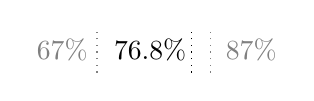
\begin{tikzpicture}[baseline=0.8ex]
    \begin{axis}[hide axis,clip=false,
	xmin=0.67,xmax=0.87,xlabel={X},
	ymin=-1,ymax=1,
	x=12cm, y=0.8em,
	]
\node [gray] at (axis cs: 0.67, 0) {$67\%$};
\node [black] at (axis cs: 0.763, 0) {$76.8\%$};
\node [gray] at (axis cs: 0.87, 0) {$87\%$};
\addplot[gray, dotted] coordinates {(0.7068, -1) (0.7068, 1)};
\addplot[gray, dotted] coordinates {(0.8268, -1) (0.8268, 1)};
\addplot[black, dotted] coordinates {(0.8068, -1) (0.8068, 1)};
    \end{axis}
\end{tikzpicture}
}


%\renewcommand{\arraystretch}{1.5}

However, when the number of known negatives is large, it may be useful to reverse our approach, i.e., start from the rank distribution of known negatives. To do so, we can essentially flip all known class labels, use $\bar{\pfrac}=1-\pfrac$ and adjust the resulting contingency tables accordingly.%, that is make the following changes: $\TP \rightarrow \FP$, $\FP\rightarrow\TP$, $\TN\rightarrow\FN$ and $\FN\rightarrow\TN$. 

Table~\ref{parameffects-both} shows bounds when based on known positives or known negatives (whichever are tightest). It is important to see that $|\knownneg| > |\knownpos|$ does not guarantee that performance bounds based on known negatives are tighter, because $\pfrac$ also affects the bounds. When computing performance bounds based on known negatives, overestimating $\hat{\pfrac}$ leads to underestimated bounds (since we use $\bar{\pfrac}=1-\hat{\pfrac}$) and vice versa. The effect of errors in $\hat{\pfrac}$ is opposite in bounds based on $\knownneg$.

Hence, bounds on performance metrics can be computed based primarily on known positives $\knownpos$ \emph{or} known negatives $\knownneg$. The width of the bounds depends on the combination of $|\knownpos|$ (or $|\knownneg|$) and $\pfrac$ (or $\bar{\pfrac}$) in a nontrivial way: depending on $\pfrac$, it is possible to obtain wider bounds based on known negatives, even if $|\knownneg| > |\knownpos|$ (or vice versa). In practice, we can estimate metrics based on $\knownpos$ and $\knownneg$ separately and then use whichever yields the tightest bounds, as shown in Table~\ref{parameffects-both}.

\begin{table}[!h]
\resizebox{\textwidth}{!}{
\begin{tabular}{ccccc|c|c}
\toprule
\multicolumn{3}{c}{configuration} & & \multicolumn{3}{c}{bounds on area under the ROC curve (true AUROC=$76.8\%$)} \\ \cline{1-3} \cline{5-7}
$\frac{|\knownpos|}{|\bothpos|}$	& $\frac{|\knownneg|}{|\mathcal{N}_\Omega|}$ & $\pfrac$ & & $\hat{\pfrac}\ /\ \pfrac = 0.8$ & $\hat{\pfrac}\ /\ \pfrac = 1.0$  & $\hat{\pfrac}\ /\ \pfrac = 1.2$ \\ 
\midrule
\ifdefined\showtikzplots
10				&	0	& 15	& & \plotauc{0.7099}{0.8063}  & \plotauc{0.7163}{0.8182}  & \plotauc{0.7235}{0.8303} \\
				&	20	& 18	& & \plotauc{0.7099}{0.8062}  & \plotauc{0.7163}{0.8180}  & \plotauc{0.7235}{0.8299} \\
				&	40	& 23	& & \plotauc{0.7099}{0.8060}  & \plotauc{0.7163}{0.8176}  & \plotauc{0.7235}{0.8289} \\
				&	60	& 31	& & \plotauc{0.7099}{0.8059}  & \plotauc{0.7163}{0.8059}  & \plotauc{0.7235}{0.8270} \\
				&	80	& 47	& & \plotauc{0.7099}{0.8055}  & \plotauc{0.7163}{0.8055}  & \plotauc{0.7235}{0.8160} \\
 & & & & \plotauclabels & \plotauclabels  & \plotauclabels \\
30				&	0	& 12	& & \plotauc{0.7328}{0.7732}  & \plotauc{0.7378}{0.7823}  & \plotauc{0.7434}{0.7915} \\
				&	20	& 15	& & \plotauc{0.7328}{0.7732}  & \plotauc{0.7378}{0.7823}  & \plotauc{0.7434}{0.7915} \\
				&	40	& 19	& & \plotauc{0.7328}{0.7732}  & \plotauc{0.7378}{0.7823}  & \plotauc{0.7434}{0.7914} \\
				&	60	& 26	& & \plotauc{0.7328}{0.7732}  & \plotauc{0.7378}{0.7823}  & \plotauc{0.7434}{0.7914} \\
				&	80	& 41	& & \plotauc{0.7328}{0.7732}  & \plotauc{0.7378}{0.7822}  & \plotauc{0.7434}{0.7907} \\
 & & & & \plotauclabels & \plotauclabels  & \plotauclabels \\
50				&	0	& 9	& & \plotauc{0.7455}{0.7682}  & \plotauc{0.7502}{0.7739}  & \plotauc{0.7573}{0.7807} \\
				&	20	& 11	& & \plotauc{0.7455}{0.7682}  & \plotauc{0.7542}{0.7779}  & \plotauc{0.7573}{0.7807} \\
				&	40	& 14	& & \plotauc{0.7455}{0.7682}  & \plotauc{0.7542}{0.7779}  & \plotauc{0.7573}{0.7807} \\
				&	60	& 20	& & \plotauc{0.7455}{0.7682}  & \plotauc{0.7542}{0.7779}  & \plotauc{0.7573}{0.7807} \\
				&	80	& 33	& & \plotauc{0.7455}{0.7682}  & \plotauc{0.7542}{0.7779}  & \plotauc{0.7573}{0.7804} \\
 & & & & \plotauclabels & \plotauclabels  & \plotauclabels \\
70				&	0	& 6	& & \plotauc{0.7533}{0.7646}  & \plotauc{0.7594}{0.7727}  & \plotauc{0.7676}{0.7778} \\
				&	20	& 7	& & \plotauc{0.7533}{0.7646}  & \plotauc{0.7594}{0.7727}  & \plotauc{0.7676}{0.7778} \\
				&	40	& 9	& & \plotauc{0.7533}{0.7646}  & \plotauc{0.7594}{0.7727}  & \plotauc{0.7676}{0.7778} \\
				&	60	& 13	& & \plotauc{0.7533}{0.7646}  & \plotauc{0.7594}{0.7727}  & \plotauc{0.7676}{0.7778} \\
				&	80	& 23	& & \plotauc{0.7533}{0.7646}  & \plotauc{0.7594}{0.7727}  & \plotauc{0.7676}{0.7778} \\
\fi
\bottomrule
\end{tabular}
}
\caption[]{Estimated bounds on AUROC under different configurations. The total data set comprises $2,000$ positives and $10,000$ negatives. We varied the fraction of known positives and known negatives, which also implies changing $\pfrac$. All entries in the table are in percentages. We used three estimates for $\hat{\pfrac}$, namely an underestimate, the correct value and an overestimate (left to right). \newline
Legend:
\begin{tikzpicture}[baseline=-0.5ex] \draw [color=black, thick, dashed] (0, 0) -- (0.5, 0); \end{tikzpicture} true AUROC, 

\begin{tikzpicture}[baseline=-0.5ex] \draw [color=cyan!80!black, opacity=0.8] (0, -0.15) rectangle (0.7, 0.25); 
\fill [color=cyan!80!black, opacity=0.4] (0, -0.15) rectangle (0.7, 0.25); \end{tikzpicture} bounds based on known positives.
}
\label{parameffects-posonly}
\end{table}


\begin{table}[!h]
\resizebox{\textwidth}{!}{
\begin{tabular}{ccccc|c|c}
\toprule
\multicolumn{3}{c}{configuration} & & \multicolumn{3}{c}{bounds on area under the ROC curve (true AUROC=$76.8\%$)} \\ \cline{1-3} \cline{5-7}
$\frac{|\knownpos|}{|\bothpos|}$	& $\frac{|\knownneg|}{|\mathcal{N}_\Omega|}$ & $\pfrac$ & & $\hat{\pfrac}\ /\ \pfrac = 0.8$ & $\hat{\pfrac}\ /\ \pfrac = 1.0$  & $\hat{\pfrac}\ /\ \pfrac = 1.2$ \\ 
\midrule
\ifdefined\showtikzplots
10 & 0 & 15 & & \plotauccolor{0.7081}{0.8044}{cyan} & \plotauccolor{0.7143}{0.8160}{cyan} & \plotauccolor{0.7214}{0.8277}{cyan} \\
 & 20 & 18 & & \plotauccolor{0.7081}{0.8043}{cyan} & \plotauccolor{0.7143}{0.8159}{cyan} & \plotauccolor{0.7214}{0.8274}{cyan} \\
 & 40 & 23 & & \plotauccolor{0.7950}{0.8724}{red} & \plotauccolor{0.7420}{0.8215}{red} & \plotauccolor{0.7067}{0.7742}{red} \\
 & 60 & 31 & & \plotauccolor{0.8106}{0.8531}{red} & \plotauccolor{0.7564}{0.8003}{red} & \plotauccolor{0.7182}{0.7538}{red} \\
 & 80 & 47 & & \plotauccolor{0.8072}{0.8287}{red} & \plotauccolor{0.7534}{0.7729}{red} & \plotauccolor{0.7165}{0.7301}{red} \\
 & & & & \plotauclabels & \plotauclabels  & \plotauclabels \\
30 & 0 & 12 & & \plotauccolor{0.7367}{0.7803}{cyan} & \plotauccolor{0.7417}{0.7896}{cyan} & \plotauccolor{0.7474}{0.7989}{cyan} \\
 & 20 & 14 & & \plotauccolor{0.7367}{0.7802}{cyan} & \plotauccolor{0.7417}{0.7896}{cyan} & \plotauccolor{0.7474}{0.7988}{cyan} \\
 & 40 & 18 & & \plotauccolor{0.7367}{0.7802}{cyan} & \plotauccolor{0.7417}{0.7895}{cyan} & \plotauccolor{0.7474}{0.7987}{cyan} \\
 & 60 & 25 & & \plotauccolor{0.7964}{0.8347}{red} & \plotauccolor{0.7567}{0.7996}{red} & \plotauccolor{0.7256}{0.7638}{red} \\
 & 80 & 41 & & \plotauccolor{0.7935}{0.8125}{red} & \plotauccolor{0.7539}{0.7727}{red} & \plotauccolor{0.7235}{0.7386}{red} \\
 & & & & \plotauclabels & \plotauclabels  & \plotauclabels \\
50 & 0 & 9 & & \plotauccolor{0.7488}{0.7706}{cyan} & \plotauccolor{0.7524}{0.7773}{cyan} & \plotauccolor{0.7564}{0.7841}{cyan} \\
 & 20 & 11 & & \plotauccolor{0.7488}{0.7706}{cyan} & \plotauccolor{0.7524}{0.7773}{cyan} & \plotauccolor{0.7564}{0.7841}{cyan} \\
 & 40 & 14 & & \plotauccolor{0.7488}{0.7706}{cyan} & \plotauccolor{0.7524}{0.7773}{cyan} & \plotauccolor{0.7564}{0.7840}{cyan} \\
 & 60 & 20 & & \plotauccolor{0.7488}{0.7706}{cyan} & \plotauccolor{0.7524}{0.7773}{cyan} & \plotauccolor{0.7564}{0.7840}{cyan} \\
 & 80 & 33 & & \plotauccolor{0.7807}{0.7992}{red} & \plotauccolor{0.7537}{0.7724}{red} & \plotauccolor{0.7313}{0.7475}{red} \\
 & & & & \plotauclabels & \plotauclabels  & \plotauclabels \\
70 & 0 & 5 & & \plotauccolor{0.7554}{0.7667}{cyan} & \plotauccolor{0.7576}{0.7709}{cyan} & \plotauccolor{0.7599}{0.7751}{cyan} \\
 & 20 & 6 & & \plotauccolor{0.7554}{0.7667}{cyan} & \plotauccolor{0.7576}{0.7709}{cyan} & \plotauccolor{0.7599}{0.7751}{cyan} \\
 & 40 & 9 & & \plotauccolor{0.7554}{0.7667}{cyan} & \plotauccolor{0.7576}{0.7709}{cyan} & \plotauccolor{0.7599}{0.7751}{cyan} \\
 & 60 & 13 & & \plotauccolor{0.7554}{0.7667}{cyan} & \plotauccolor{0.7576}{0.7709}{cyan} & \plotauccolor{0.7599}{0.7751}{cyan} \\
 & 80 & 23 & & \plotauccolor{0.7554}{0.7667}{cyan} & \plotauccolor{0.7576}{0.7709}{cyan} & \plotauccolor{0.7599}{0.7751}{cyan} \\
\fi
\bottomrule
\end{tabular}
}
\caption[]{Estimated bounds on AUROC under different configurations. The total data set comprises $2,000$ positives and $10,000$ negatives. We varied the fraction of known positives and known negatives, which also implies changing $\pfrac$. All entries in the table are in percentages. We used three estimates for $\hat{\pfrac}$, namely an underestimate, the correct value and an overestimate (left to right). In this table, we computed bounds based on known positives and known negatives (separately) and report the tightest confidence interval each time. \newline
Legend: 
\begin{tikzpicture}[baseline=-0.5ex] \draw [color=black, thick, dashed] (0, 0) -- (0.5, 0); \end{tikzpicture} true AUROC, bounds based on 

\begin{tikzpicture}[baseline=-0.5ex] \draw [color=cyan!80!black, opacity=0.8] (0, -0.15) rectangle (0.7, 0.25); 
\fill [color=cyan!80!black, opacity=0.4] (0, -0.15) rectangle (0.7, 0.25); \end{tikzpicture} known positives and 

\begin{tikzpicture}[baseline=-0.5ex] \draw [color=red!80!black, opacity=0.8] (0, -0.15) rectangle (0.7, 0.25); 
\fill [color=red!80!black, opacity=0.4] (0, -0.15) rectangle (0.7, 0.25); \end{tikzpicture} known negatives.}
\label{parameffects-both}
\end{table}


%\section{Proofs}


\end{document}
